\chapter{The BONuS12 Experiment}
\label{ch:bonus}
The Barely Off-shell Nucleon Structure experiment at 12 GeV energy (BONuS12) used a electron scattering off a neutron in a deuterium target to detect low momentum (less than 100 MeV/c) backward-going (angles above 100$^{\circ}$) spectator protons in a Radial Time Projection Chamber (RTPC). The spectator proton was detected in coincidence with the scattered electron in order to establish the semi-inclusive DIS interaction $D(e,e',p_s)X$ that BONuS12 will use to extract the structure function ratio $F_2^n/F_2^p$.

BONuS12 was conducted at the Thomas Jefferson National Laboratory (JLab) in Newport News, Virginia. JLab was founded in 1984 with the intent of studying the structure of nuclear matter. The unique accelerator that was built at JLab, called the Continuous Electron Beam Accelerator Facility (CEBAF), allowed for the realization of that intent by providing the ability to probe atomic nuclei at the quark level. In order to understand the BONuS12 experiment, we must first understand CEBAF and the Hall B spectrometer where the BONuS12 RTPC was installed. Then we will discuss the RTPC design, components, and construction.

\begin{figure}[h!]
	\centering
	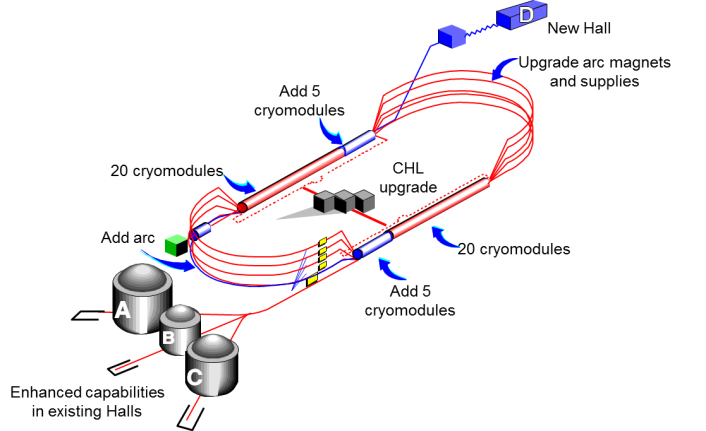
\includegraphics[width=0.8\linewidth]{figures/cebaf.png}
	\caption[CEBAF upgraded for the 12 GeV era.]{CEBAF upgraded for the 12 GeV era \cite{pres:CEBAF}.}
	\label{fig:cebaf}
\end{figure}

\section{Continuous Electron Beam Accelerator Facility}
The construction of the Continuous Electron Beam Accelerator Facility (CEBAF) was completed in 1994. It originally consisted of two antiparallel linear accelerators (LINACs) connected by nine recirculation arcs that accelerated electrons to an energy of 6 GeV at a current of up to 300 \textmu A. In 2004, JLab began an energy upgrade that would allow CEBAF to supply electrons up to 12 GeV. The same framework used for the 6 GeV accelerator was used for the 12 GeV era. That is, each pass around the accelerator increased the electron energy, which was 1-1.2 GeV/pass during the 6 GeV era \cite{clasnote:CEBAF} and 2.2 GeV/pass after the 12 GeV upgrade. Originally, that meant 5 passes would produce 6 GeV electrons before they were fed into the three existing experimental halls ($i.e.$ Hall A, Hall B, and Hall C). In addition to the energy upgrade, a new experimental hall was built ($i.e.$ Hall D). Now, 5 passes creates a 10.5 GeV electron beam to Halls A, B and C. Hall D received electrons from 5.5 passes around the accelerator creating the 12 GeV electron beam energy. As Fig. \ref{fig:cebaf} shows, the upgrade consisted of 5 additional cryomodules in each LINAC, an additional recirculation arc, increased capacity of the Central Helium Liquefier (CHL), and improvements in the curving magnets.\cite{pres:CEBAF}

The electrons are accelerated in CEBAF by way of the LINACs. These LINACs contain a set of superconducting Niobium accelerating cavities with electromagnetic fields that oscillate at a frequency of 1.5 GHz. Electrons are injected in bunches into the accelerator with an energy of 45 MeV at the same frequency as the cavities every 0.7 ns.\cite{clasnote:CEBAF} These electrons then circulate around, increasing in energy each pass through the LINACs. Once the desired energy for a given hall is reached, every 2.1 ns magnetic fields inside the arcs force the electrons into specific central trajectories that guides them into that hall. The beam is considered ``continuous" because the high operating frequency has a maximum current of 200 \textmu A. Each hall contains a device called a Faraday Cup (FC) located at the end of the beam line that measures the total amount of charge accumulated, which allows for monitoring of the number of electrons impacting its target during the taking of data.
 
\section{CEBAF Large Acceptance Spectrometer}
Once the electrons are accelerated to a desired energy, they are received by the halls, where they are directed towards a target. The scattered particles enter each hall's spectrometer, while beam electrons that do not scatter off the target hit the FC. A spectrometer is an instrument (or collection of instruments) that measures and analyzes a range (or spectrum) of processes or reactions. In scattering experiments, a spectrometer separates particles in space via some physical property, and the magnets in the spectrometer separates particles based on momentum. Because BONuS12 will operate in Hall B, here we will focus on the components and operation of Hall B's spectrometer, called the CEBAF Large Acceptance Spectrometer at 12 GeV energy (or CLAS12). As the name suggests, CLAS12 is an evolution of CLAS6 (or just CLAS as it was known before talk of the energy upgrade), which was the original spectrometer built for Hall B. 

\begin{figure}[h!]
	\centering
	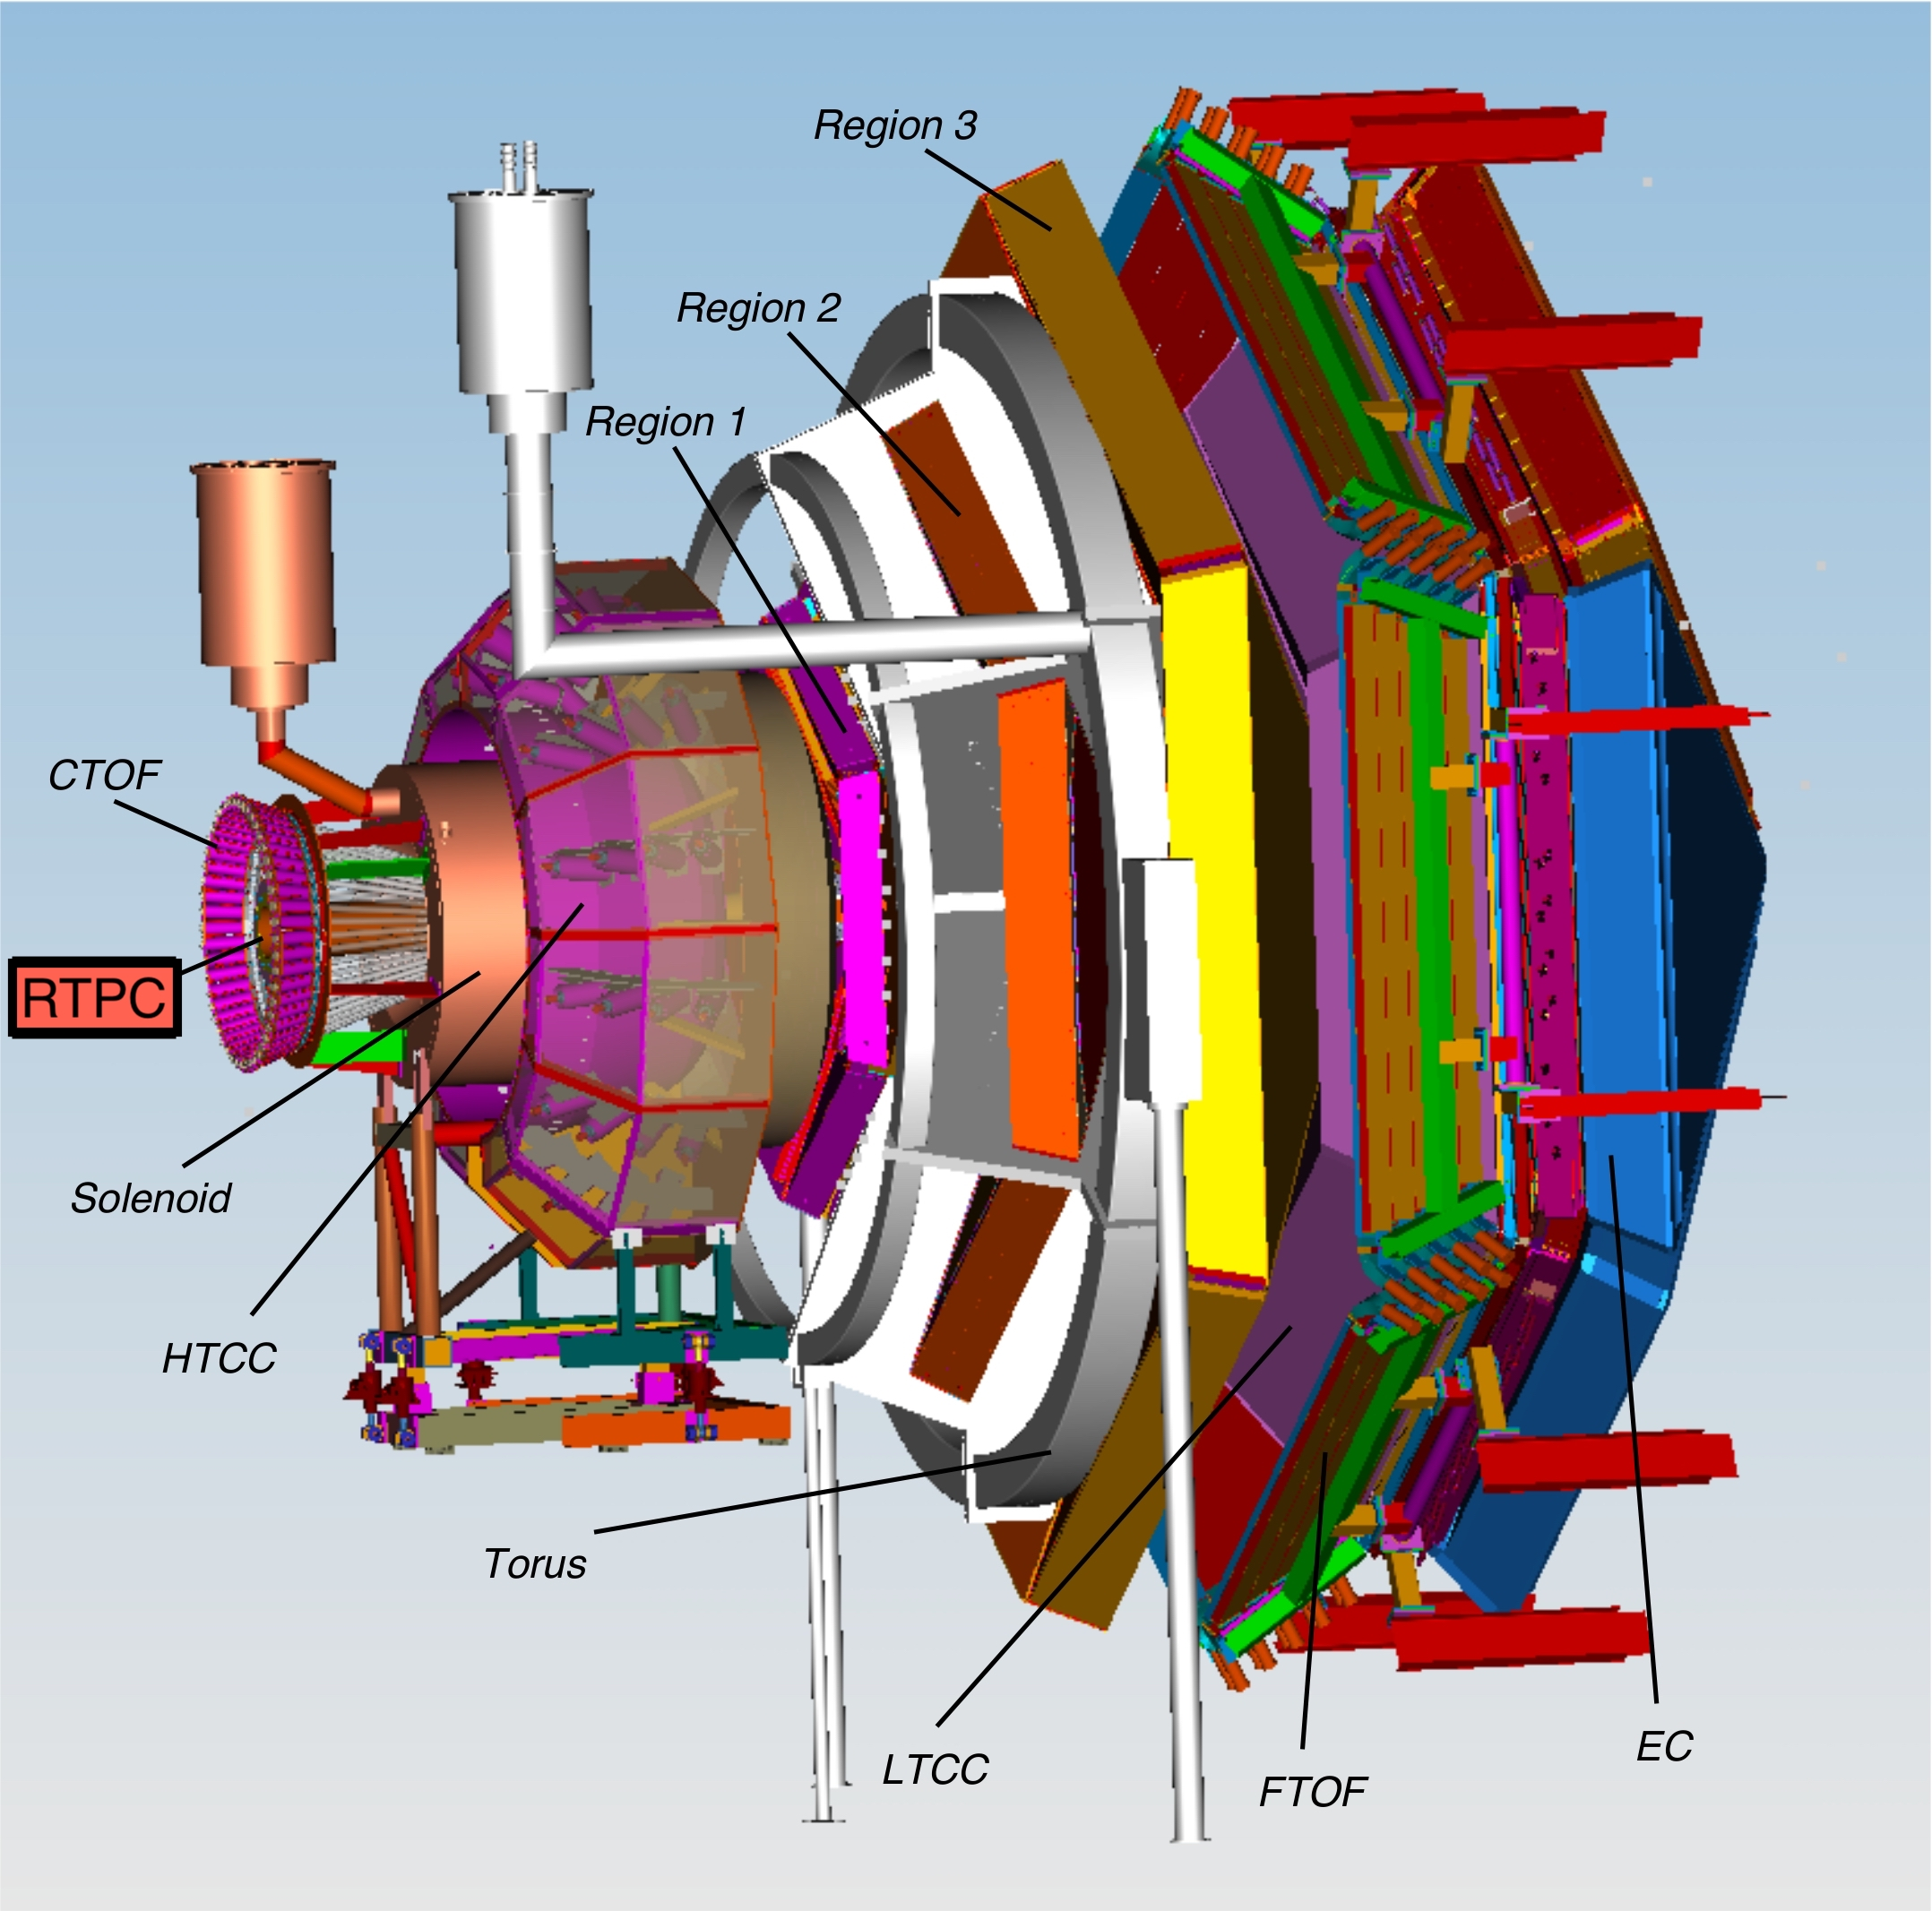
\includegraphics[width=0.8\linewidth]{figures/clas12.png}
	\caption[The CEBAF Large Acceptance Spectrometer at 12 GeV (CLAS12).]{The CEBAF Large Acceptance Spectrometer at 12 GeV (CLAS12) \cite{pres:CEBAF}.}
	\label{fig:clas12}
\end{figure}

CLAS12 (see Fig. \ref{fig:clas12}) consists of two major groups of detectors, which together allow for detection and identification of particles over a large scattering angle, thus the ``Large Acceptance" in the name CLAS12. The Forward Detector (FD) covers scattering angles of between 5 and 40 degrees, and consists of a torus magnet, Cherenkov counters, a time of flight detector, drift chambers and electromagnetic calorimeter. The other group of detectors is known as the Central Detector (CD), and covers scattering angles between 40 and 125 degrees.\cite{CLAS12} The CD consists of a solenoid magnet, time of flight detector and finally, the BONuS12 RTPC. We will discuss each of these detectors, with a bit more focus on the RTPC.

\subsection{Torus Magnet}
The torus magnet is comprised of six superconducting coils arranged symmetrically around the beamline to create an azimuthally-symmetric magnetic field up to 3.5 T. The coils are cooled to an operating temperature of 4.5 K by liquid helium.\cite{clas12:mags} The shape of the coils was designed to create a field that increases near the center, which provides the desired resolution as a function of $\theta$.

The purpose of the magnetic field is to curve the tracks of charged particles without changing their azimuthal ($\phi$) angle. This curvature allows for the increased capability of particle identification by separating particles by their momentum. Its open structure allows for long path lengths for both charged and neutral particles, which also contributes to particle identification through time-of-flight measurements.

\subsection{Cherenkov Counters}
When a charged particle moves through a dialectric\footnote{A dialectric is any insulator that can be polarized when an electric field is applied.} with a speed greater than the phase velocity of light in that medium, electromagnetic radiation ($i.e.$ light) is emitted. This is known as Cherenkov radiation. By changing the refractive index of that medium, the threshold for emission of that light is modified. The threshold of the particle energy is given by \cite{clas12:HTCC}
\begin{equation}
E = \frac{m}{\sqrt{1-\beta^2}} = m\frac{n^2}{n^2-1},
\end{equation}
where $m$ is the mass of the particle, $\beta$ is its speed in units of the speed of light, and $n$ is the index of refraction of the medium. This effect allows for the distinction of particles having the same momentum but different mass. By using a material with a specific refractive index, a heavier particle may not produce Cherenkov light, but a lighter particle may.

\begin{wrapfigure}{L}{0.35\linewidth}
	\centering
	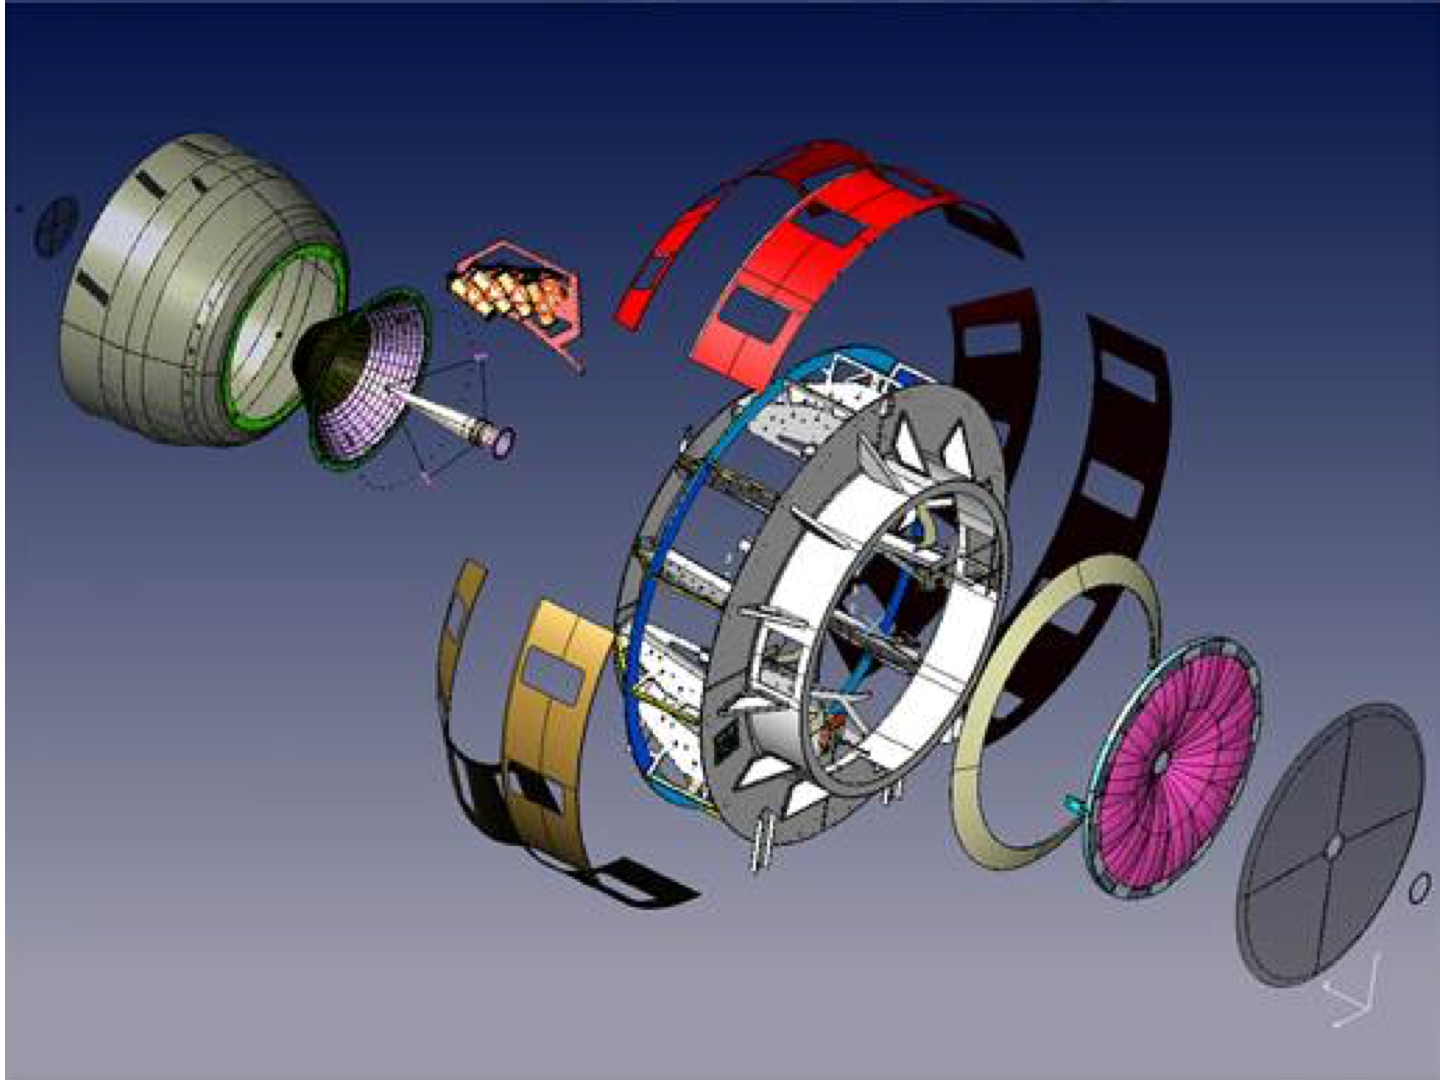
\includegraphics[width=0.9\linewidth]{figures/htcc.png}
	\caption[The High Threshold Cerenkov Counter.]{\label{fig:htcc}The High Threshold Cerenkov Counter \cite{clas12:HTCC}.}
\end{wrapfigure}
CLAS12 contains two detectors that exploit this Cherenkov effect. The High Threshold Cherenkov Counter (HTCC seen exploded in Fig. \ref{fig:htcc}) is between the target and the first region of the Drift Chambers. It discriminates electrons from charged pions, kaons, and protons by being filled with CO$_2$.\cite{clas12:HTCC} This gas has an index of refraction $n=1.00041$, which forces pions above 4.9 GeV to produce light. If the particle has an energy below this threshold and it produces light, it is an electron. The other Cherenkov detector is the Low Threshold Cerenkov Counter (LTCC), which sits between Region 3 of the Drift Chambers and the Forward Time of Flight detector. It is filled with C$_4$F$_{12}$, which allows for the detection of pions above a momentum of 3.5 GeV where only pions produce Cherenkov light.\cite{clas12:LTCC}

\subsection{Drift Chambers}
There are three regions of Drift Chambers (DC) that collectively allow for the reconstruction of charged particle trajectories. The first region is located in front of the Torus Magnet outside of the field. Region 2 is between the coils in the high field region. The third region is after the torus, but feels a small magnetic field from the coils. Each region is made of six triangular sectors, which consists of small wires under tension and at high voltage. 

\begin{figure}[H]
	\centering
	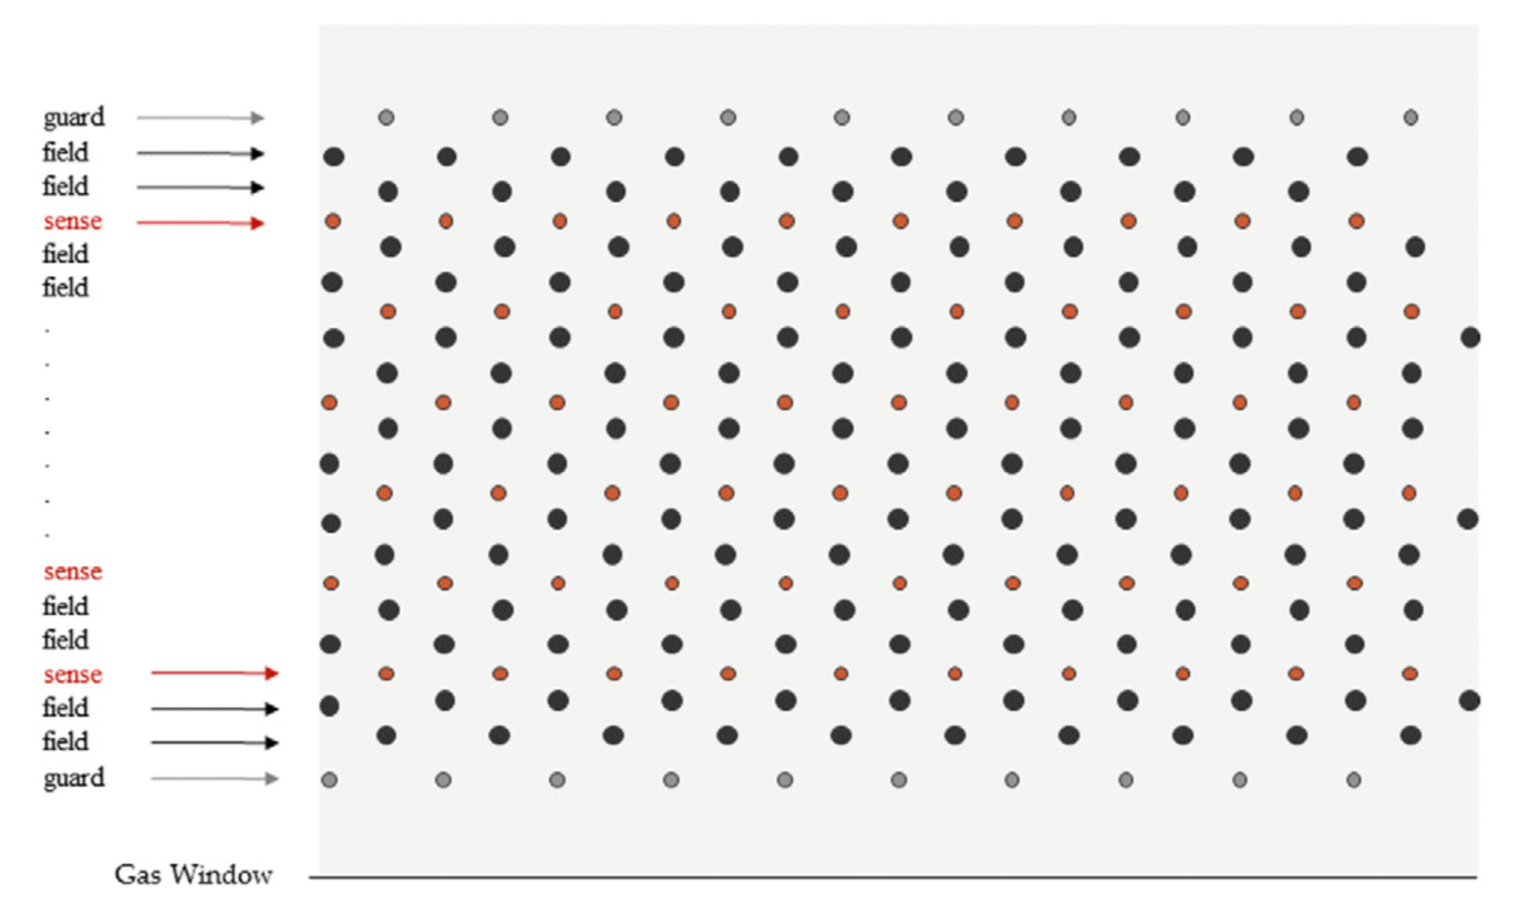
\includegraphics[width=0.8\linewidth]{figures/dc_wires.png}
	\caption[Hexagonal wire layout for the drift chamber.]{Hexagonal wire layout for the drift chamber \cite{clas12:DC}.}
	\label{fig:dc_wires}
\end{figure}

Within the sectors of the DC there are hundreds of wires. Sense wires are located in between field wires all in a hexagonal pattern (see Fig. \ref{fig:dc_wires}). When a charged particle travels through the DC gas mixture of 90$\%$ Argon 10$\%$ CO$_2$\cite{clas12:DC}, it ionizes the gas molecules as it passes. In the DC, these ionization electrons are accelerated to the nearest sense wire by the electric field. The accelerating electron creates an electron avalanche as it approaches the sense wire. That avalanche makes for a detectable signal on that wire.

Using the signals created by the ionization electron-ion pairs as the primary charged particle travels through the regions of the DC allows for the reconstruction of that particle's path. This information lends itself to the reconstruction of the particle momentum as well as its vertex in the target ($i.e.$ where the particle originated). This information will be vital in BONuS12 for identifying the electron created in the $eD \rightarrow e'p_sX$ process.

\subsection{Forward Time of Flight}
Two charged particles having the same momentum will travel at different speeds depending on their mass. The Forward Time of Flight detector (FTOF) measures the time of arrival of those charged particles emerging from the target. Primarily, the FTOF will help separate pions and kaons for energies below 3 GeV. Higher energies are handled by the Cherenkov counters. Because higher momentum particles scatter at lower angles, the FTOF was constructed to have better timing resolution at lower angles. That resolution can be as small as 80 ps at the more forward angles and 150 ps at larger angles ($i.e.$ over 35 degrees).\cite{clas12:FTOF}

The FTOF is made of six sectors of plastic scintillators coupled to double-sided PMT readout. Within each sector, there are three arrays of counters. Panel 1a, which covers 5 to 35 degrees in $\theta$ contains 23 counters. Panel 1b also covers angles between 5 and 35 degrees and contains 62 counters. Finally, Panel 2 has 5 counters covering only angles between 35 and 45 degrees. 

\subsection{Electromagnetic Calorimeter}
\label{sec:EC}
Electromagnetic calorimeters measure the energy of particles traveling through it that interact via the electromagnetic interaction. The EC in CLAS12 contains three layers. The preshower calorimeter (PCAL) is the first layer and is used to identify two close gammas, which will help discriminate between neutral pions and single gammas. The next two layers are the inner and outer electromagnetic calorimeters (EC$_{\mathrm{in}}$ and EC$_{\mathrm{out}}$, respectively). Both are used collectively with the PCAL to identify electrons, photons, $\pi^0 \rightarrow \gamma \gamma$, and neutrons.

\begin{figure}[h!]
	\centering
	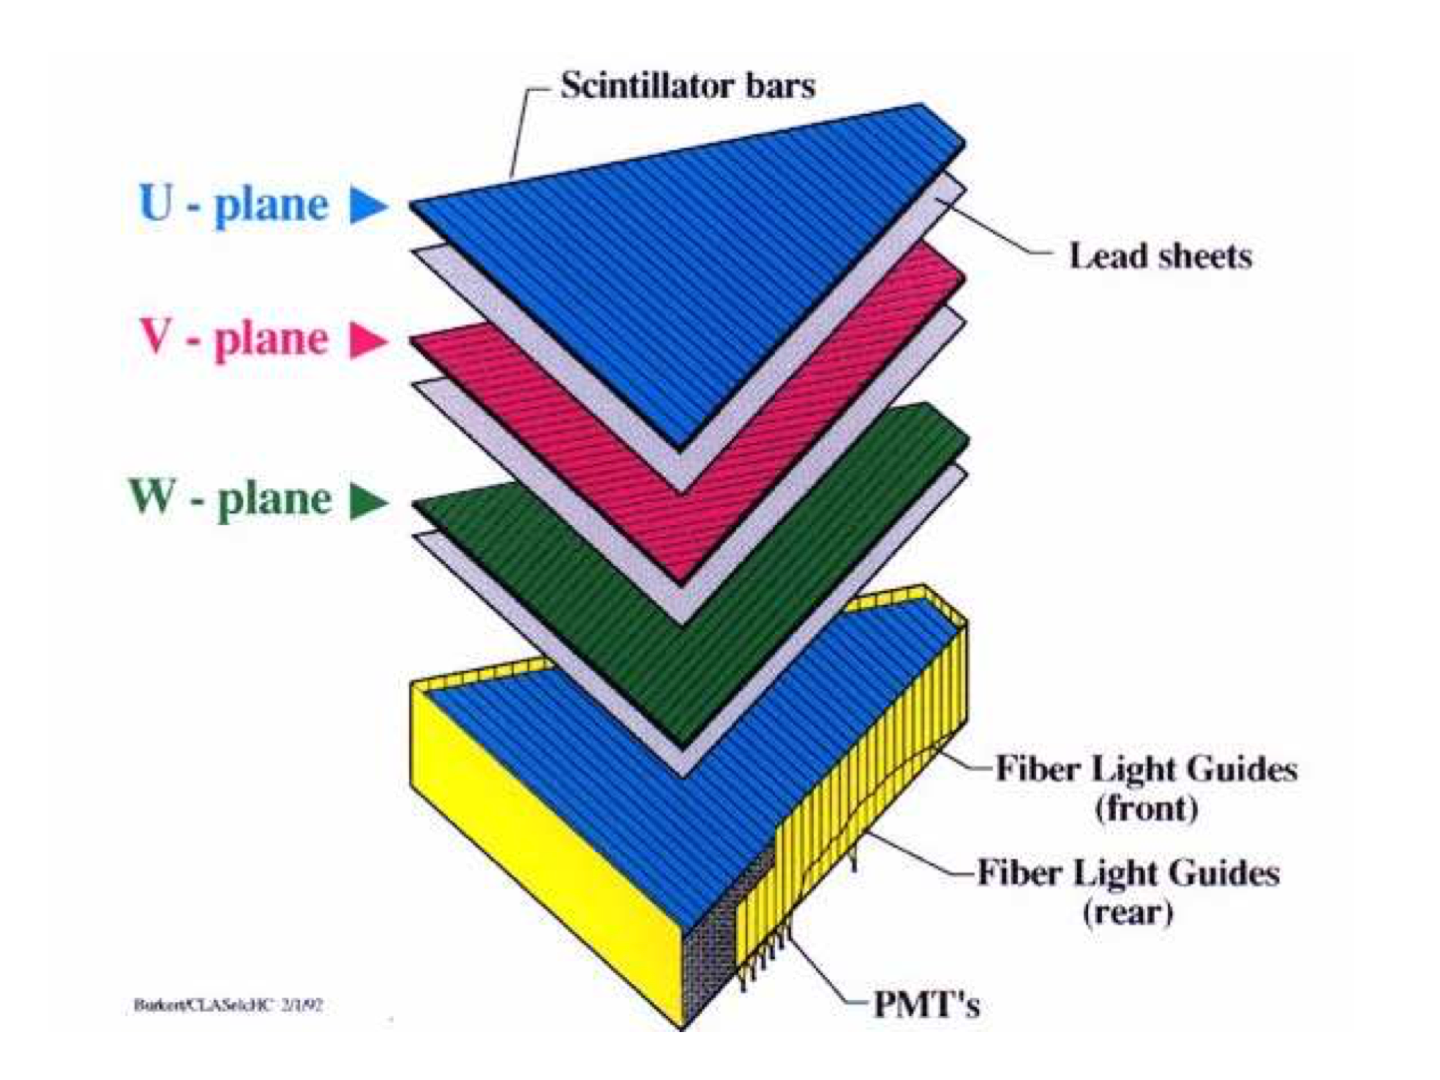
\includegraphics[width=0.8\linewidth]{figures/ecal.png}
	\caption[Exploded view of a sector of the Electromagnetic Calorimeter (EC) for CLAS12.]{Exploded view of a sector of the Electromagnetic Calorimeter (EC) for CLAS12 \cite{clasnote:EC_geo}.}
	\label{fig:ecal}
\end{figure}

The requirements of the EC are to identify electrons with energies above 0.5 GeV, and photons above 0.2 GeV, helping to reconstruct $\pi^0$ and $\eta$ particles through their neutral decays. The EC can also provide photon/neutron separation by utilizing TOF information available.

Each layer of the EC is comprised of six triangular sectors. Each sector is made of alternating layers of scintillators strips and lead sheets. The spatial-coordinate readout comes from the three planes (U, V, and W) seen in the exploded view of one sector in Fig. \ref{fig:ecal}, which each contain 36 scintillator strips that run parallel to one side of the nearly equilateral triangular sectors. Strips are rotated by 120$^{\circ}$ in each successive layer, which allows for effective translation to x, y, and z coordinates.\cite{clas12:EC}

\newpage
\subsection{Faraday Cup}
\label{sec:fc}
The Faraday Cup (FC) is a detector that measures the amount of charge deposited in it by particles. The Faraday Cup in CLAS12 sits 29.0 m downstream of the CLAS12 target and is composed of 4000 kg of lead supported on ceramic standoffs inside a vacuum chamber.\cite{CLAS12} An electrical feed-through provides a way to draw the deposited charge from the FC. The FC not only measures the integrated charge, but can also measure of the variation in charge with helicity for experiments using polarized electrons.

\subsection{Solenoid Magnet}
The solenoid magnet and the remaining two detectors to follow ($i.e.$ the Central Time of Flight and Radial Time Projection Chamber) are all members of the group known as the Central Detector. The Solenoid is a super-conducting magnet cylindrical in shape that surrounds the beam line. It is capable of producing a field of up to 5T along the beam line.\cite{clas12:mags} Charged particles experiencing this field curve in a helical trajectory, which allows for reconstruction of those trajectories and discrimination between charged and neutral particles.

The other purpose of the solenoid is to shield the Forward Detector from electron-electron collisions, called M\o ller electrons. Because the field is strongest closest to the target, most M\o ller electrons originating from the beam line are isolated by the solenoid's field to small polar angles ($\theta$) where none of the FD materials exist. The other means of protection from these M\o llers comes from a shield around the beam line located outside the Central Detector as well as a shield just in front of a small detector called the Forward Tracker, which for the BONuS12 experiment will be turned off.

\subsection{Central Time of Flight}
\begin{figure}[h!]
 	\centering
 	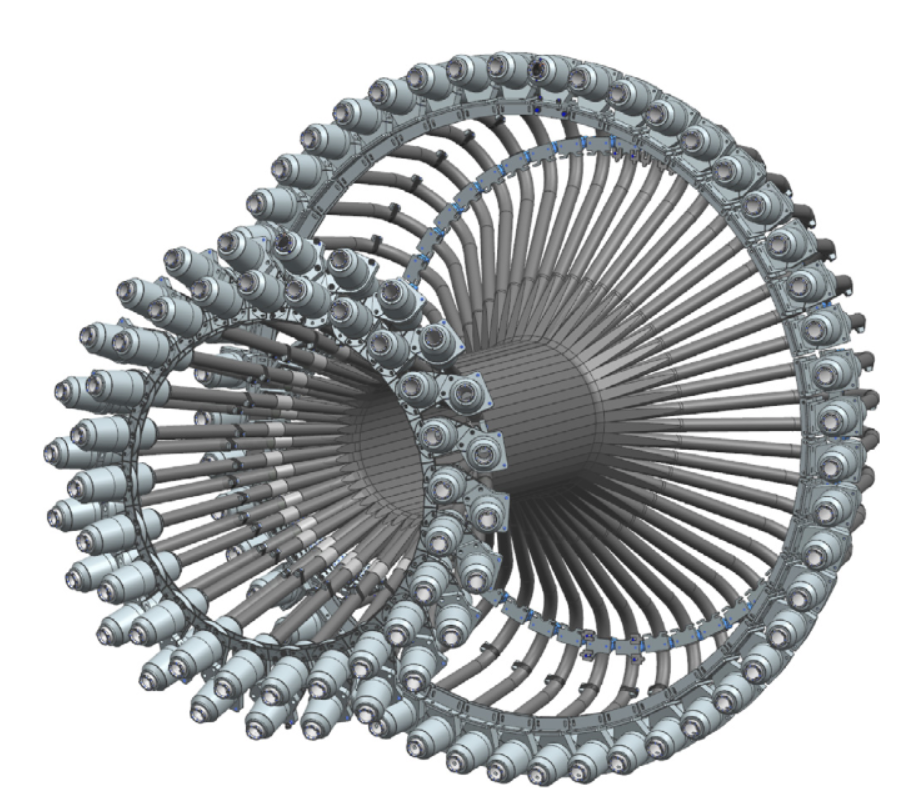
\includegraphics[width=0.8\linewidth]{figures/ctof.png}
 	\caption[The Central Time of Flight Detector.]{\label{fig:ctof}The Central Time of Flight Detector\cite{clas12:CTOF}.}
\end{figure}
The Central Time of Flight (Fig. \ref{fig:ctof}), or CTOF, is located inside the solenoid. Just as the FTOF, the CTOF measures the time of flight of particles originating at the reaction vertex. It is made of 48 scintillator bars that form a barrel and spans polar angles of 35$^{\circ}$ to 125$^{\circ}$ that surround the target with full azimuthal coverage. The scintillators are coupled on each end by magnetic-field-sensitive PMTs, which are positioned out of the solenoid field by long light guides. The resulting CTOF operates with a time resolution of 60 ps \cite{clas12:CTOF}, which was the requirement for particle identification.

\section{BONuS12 RTPC}
During Run Group F (RGF) in Hall B at JLab, all of the detectors just described will be present in addition to one more that will be located inside the solenoid magnet and CTOF. That detector is the BONuS12 Radial Time Projection Chamber (RTPC). Its purpose is to detect backward going low momentum protons by way of ionization electrons created as protons pass through the RTPC.

\subsection{Components and their Purpose}
Accelerated electrons that enter Hall B meet the 40 cm RGF target. That target measures 3 mm radially and is filled with gaseous deuterium at 7 atm pressure surrounded by a 63 \textmu m thick Kapton wall. When an electron collides with the neutron in a deuteron atom, it continues in the forward direction into the Forward Detector of CLAS12. That collision also results in the ejection of a proton that drifts radially outward into the RTPC.

\begin{figure}[h!]
	\centering
	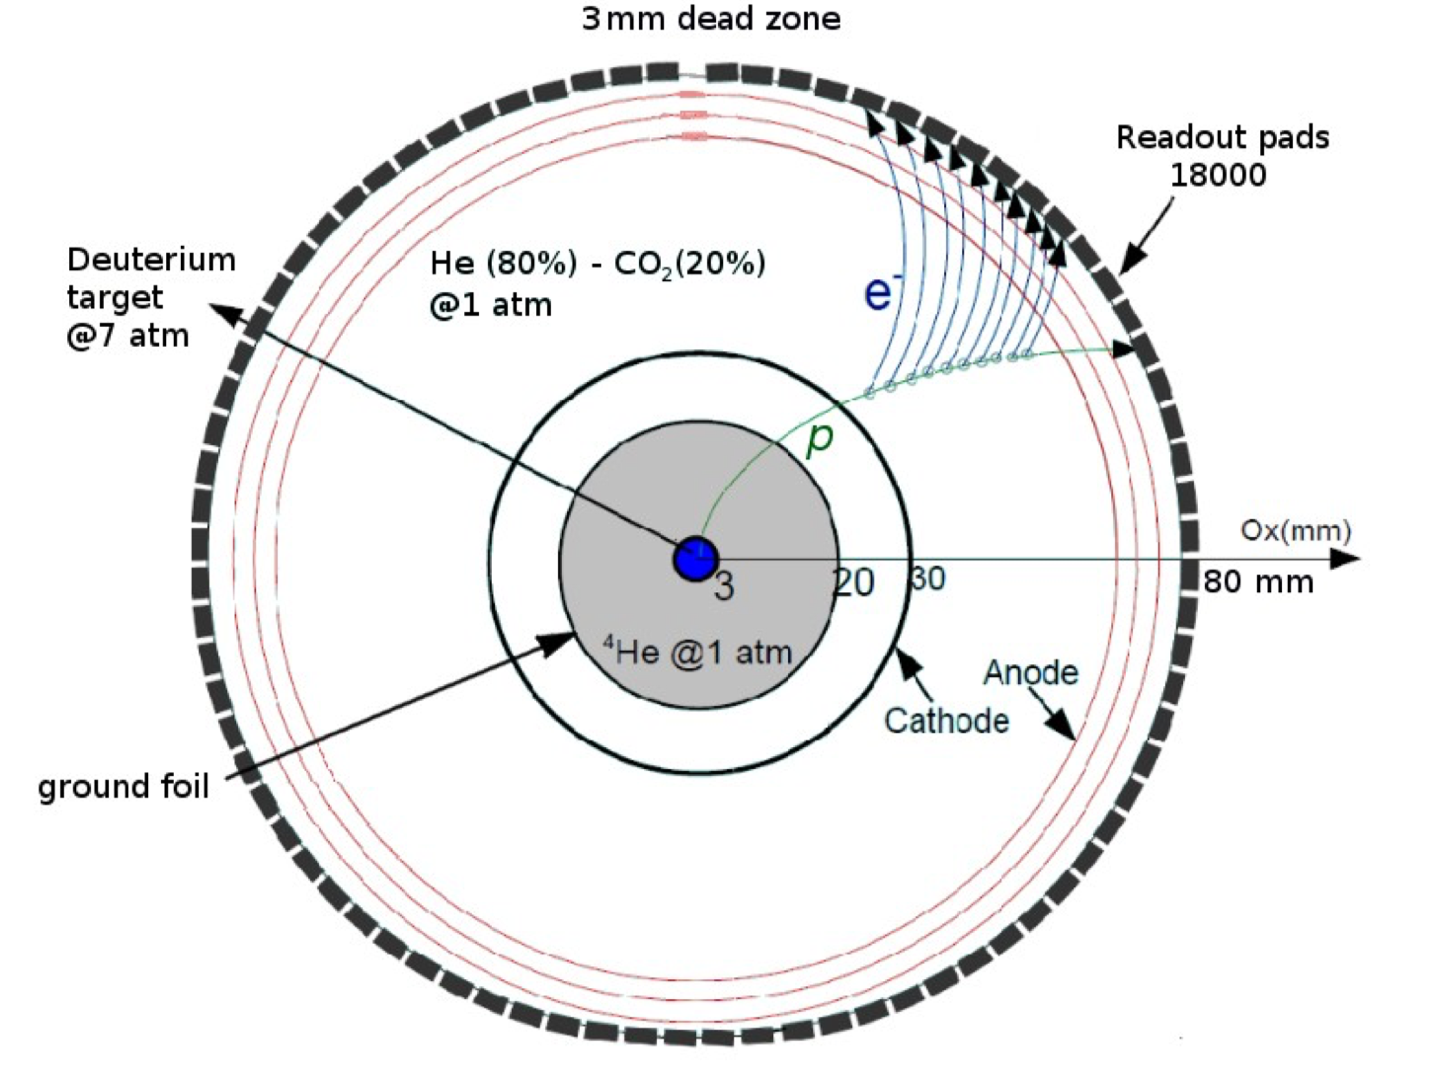
\includegraphics[width=0.8\linewidth]{figures/rtpc_op.png}
	\caption{Cross section of the RTPC showing a proton traversing the detector with ionization electrons drifting toward the readout pad board.}
	\label{fig:rtpc_op}
\end{figure}

That proton is guided toward the outer edge of the RTPC by way of an electric field created within it. That field is established with a ground foil at 2 cm and a cathode foil at 3 cm (see Fig. \ref{fig:rtpc_op}). The cathode foil is given a high negative potential and the ground foil is at zero potential to protect the target from charging up. Then the potential difference between the cathode and first Gaseous Electron Multiplier (GEM) foil at 7 cm creates an electric field through the active region of the RTPC. 

This active region between 3 and 7 cm is where the proton creates ionizations along its path outward. The region is filled with a gas mixture of 80$\%$ Helium and 20$\%$ CO$_2$, which was chosen for its fast drift times and minimal drift angle (more about this in Section \ref{sec:gas_opt}). Because of the magnetic field created by the solenoid, the proton curves in one direction as it moves outward while the ionization electrons it creates curve in the opposite direction due to their opposite charge.

\begin{figure}[h!]
	\centering
	\begin{subfigure}[b]{0.44\linewidth}
		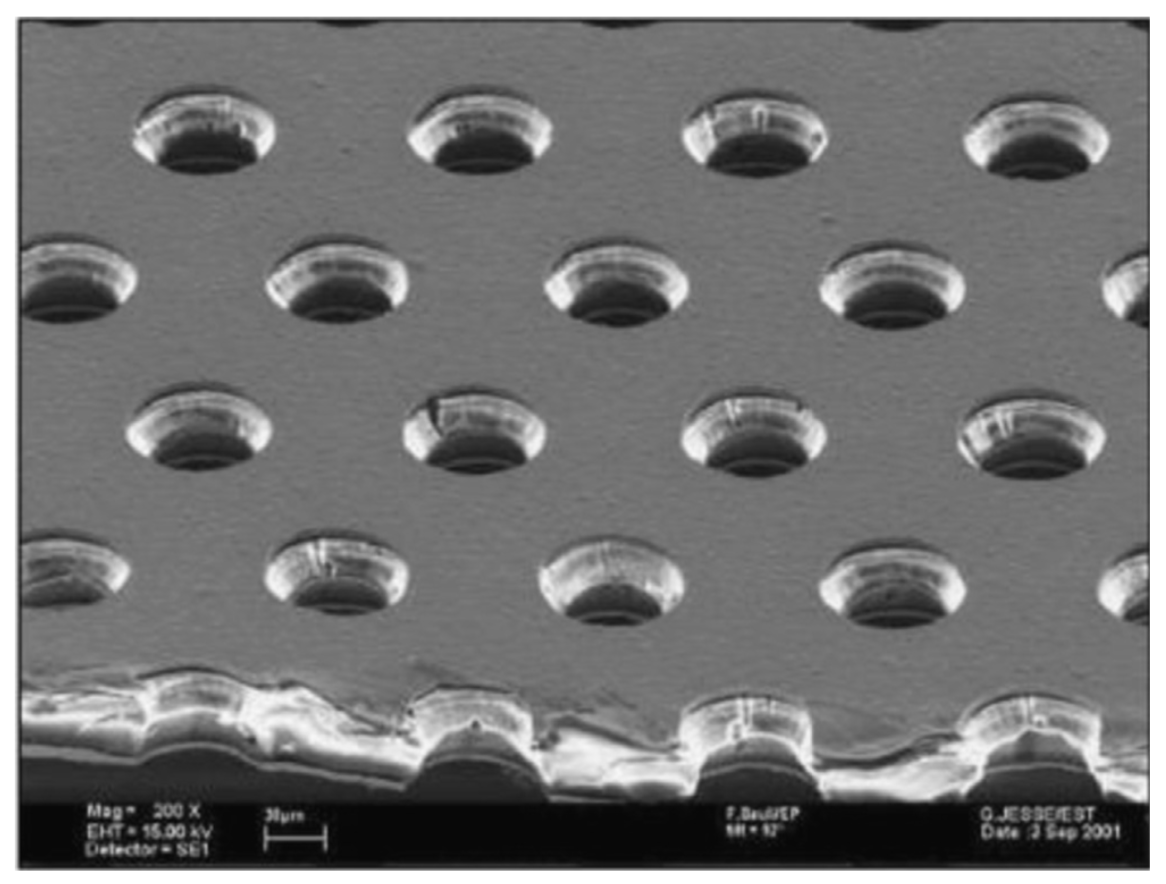
\includegraphics[width=\linewidth]{figures/gem_pic.png}
		\caption{}
	\end{subfigure}
	\begin{subfigure}[b]{0.44\textwidth}
		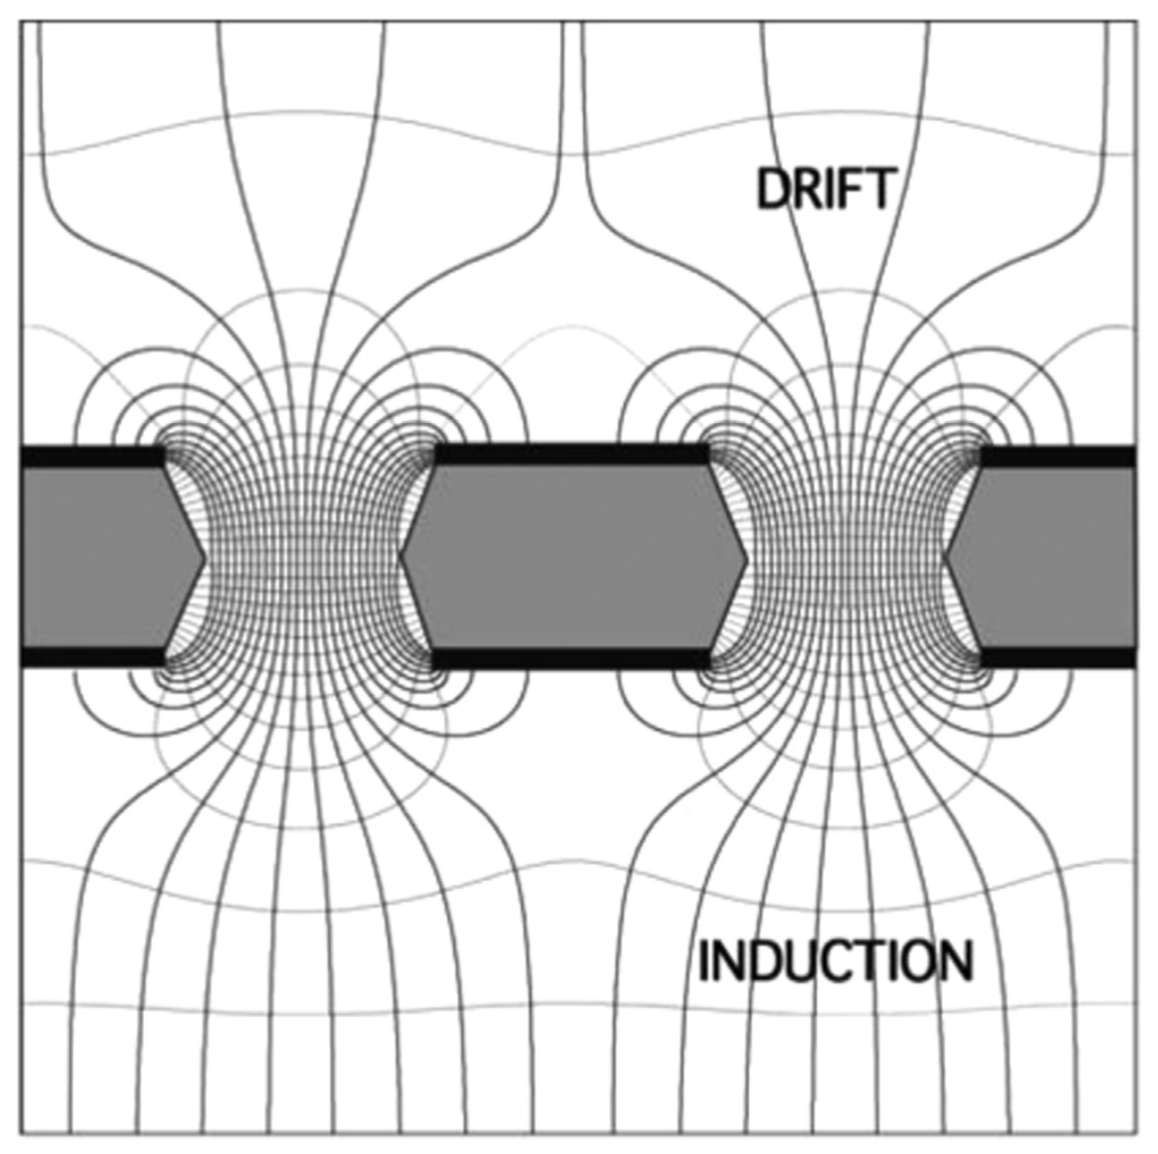
\includegraphics[width=\linewidth]{figures/gem_field.png}
		\caption{}
	\end{subfigure}
	\caption[(a) Electron microscope picture of a section of typical GEM electrode, 50 \textmu m thick. The holes pitch and diameter are 140 and 70 \textmu m, respectively. (b) Electric field in the region of the holes of a GEM electrode.]{(a) Electron microscope picture of a section of typical GEM electrode, 50 \textmu m thick. The holes pitch and diameter are 140 and 70 \textmu m, respectively\cite{GEM}. (b) Electric field in the region of the holes of a GEM electrode \cite{GEM}.}
	\label{fig:gem}
\end{figure}

Every time an ionization electron is created, it is also driven by the electric field toward the outer edge of the RTPC where there are three layers of GEM foils. That pad board provides full coverage in $\phi$ with the exception of one 3 mm dead zone down the length of the RTPC. However, because a single electron cannot be easily readout, that electron will encounter three layers of GEM foils at radii of 7 cm, 7.3 cm and 7.6 cm. Fig. \ref{fig:gem}(a) shows the surface of a GEM foil under an electron microscope. As the electron approaches the GEM foil, it is directed through one of the holes in the GEM foil by the electric field around the hole.\cite{GEM} That electric field shown in Fig. \ref{fig:gem}(b) creates an electron avalanche that multiplies the number of electrons. The GEM foils are used to amplify the number of electrons from one to something significant enough to register on the electronics. Each GEM has a gain of about 100, which means that through three GEM layers, one electron could become 1,000,000 after exiting the last layer.

\begin{figure}[h!]
	\centering
	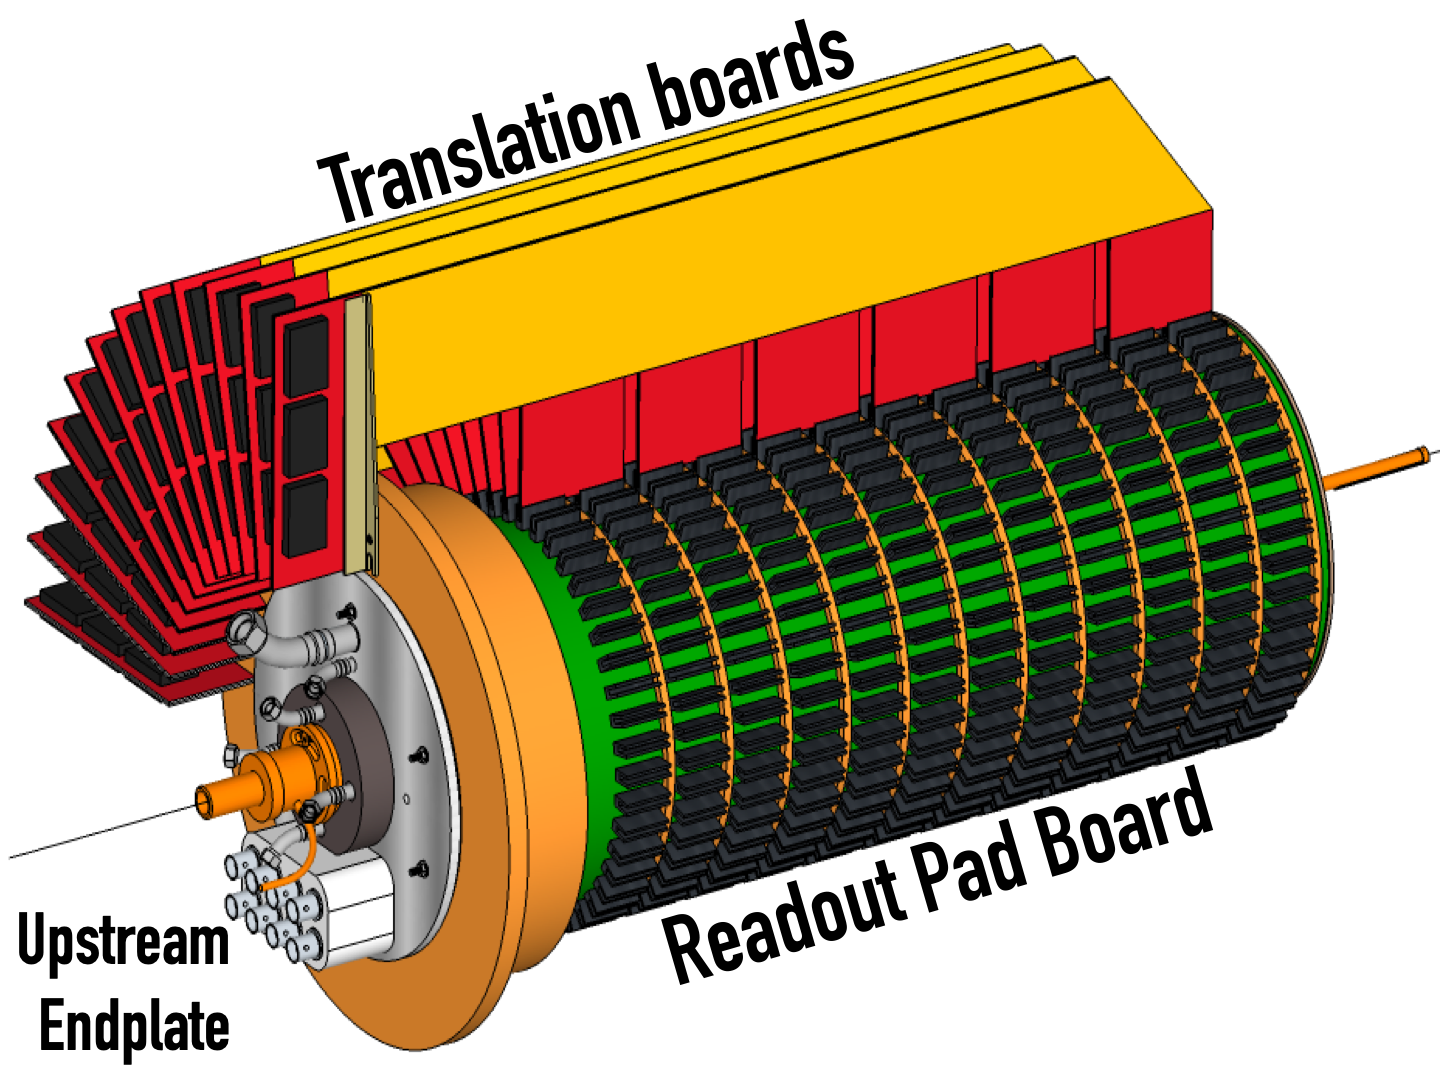
\includegraphics[width=0.8\linewidth]{figures/rtpc_design.png}
	\caption{Design of the RTPC with only one-quarter of the translation boards attached.}
	\label{fig:rtpc_design}
\end{figure}

Once this avalanche of electrons has been created by the GEMs, their final destination is the read out pad board at 8 cm. The pad board has 180 pads around $\phi$ by 96 pads in $z$ totaling 17,280 readout pads. These pads, coupled to translation boards that act as current-limiting adapter boards, read the signal that the electron avalanche makes. 

The signals from the readout pad board are driven from the translation boards to the data acquisition system (DAQ) on the front-end electrical units. The BONuS12 DAQ is begins with the Dead-timeless Readout Electronics ASIC for Micromegas (DREAM) chips. Each DREAM chip contains 64 channels. Each channel has amplifier, shaper, analog buffer, and discriminator integrated within it. The chip has a readout rate up to 20 MHz and a dead-timeless operation of up to 20 kHz. Fig. \ref{fig:dreamn} shows the layout of the DREAM chip.

\begin{figure}[h!]
	\centering
	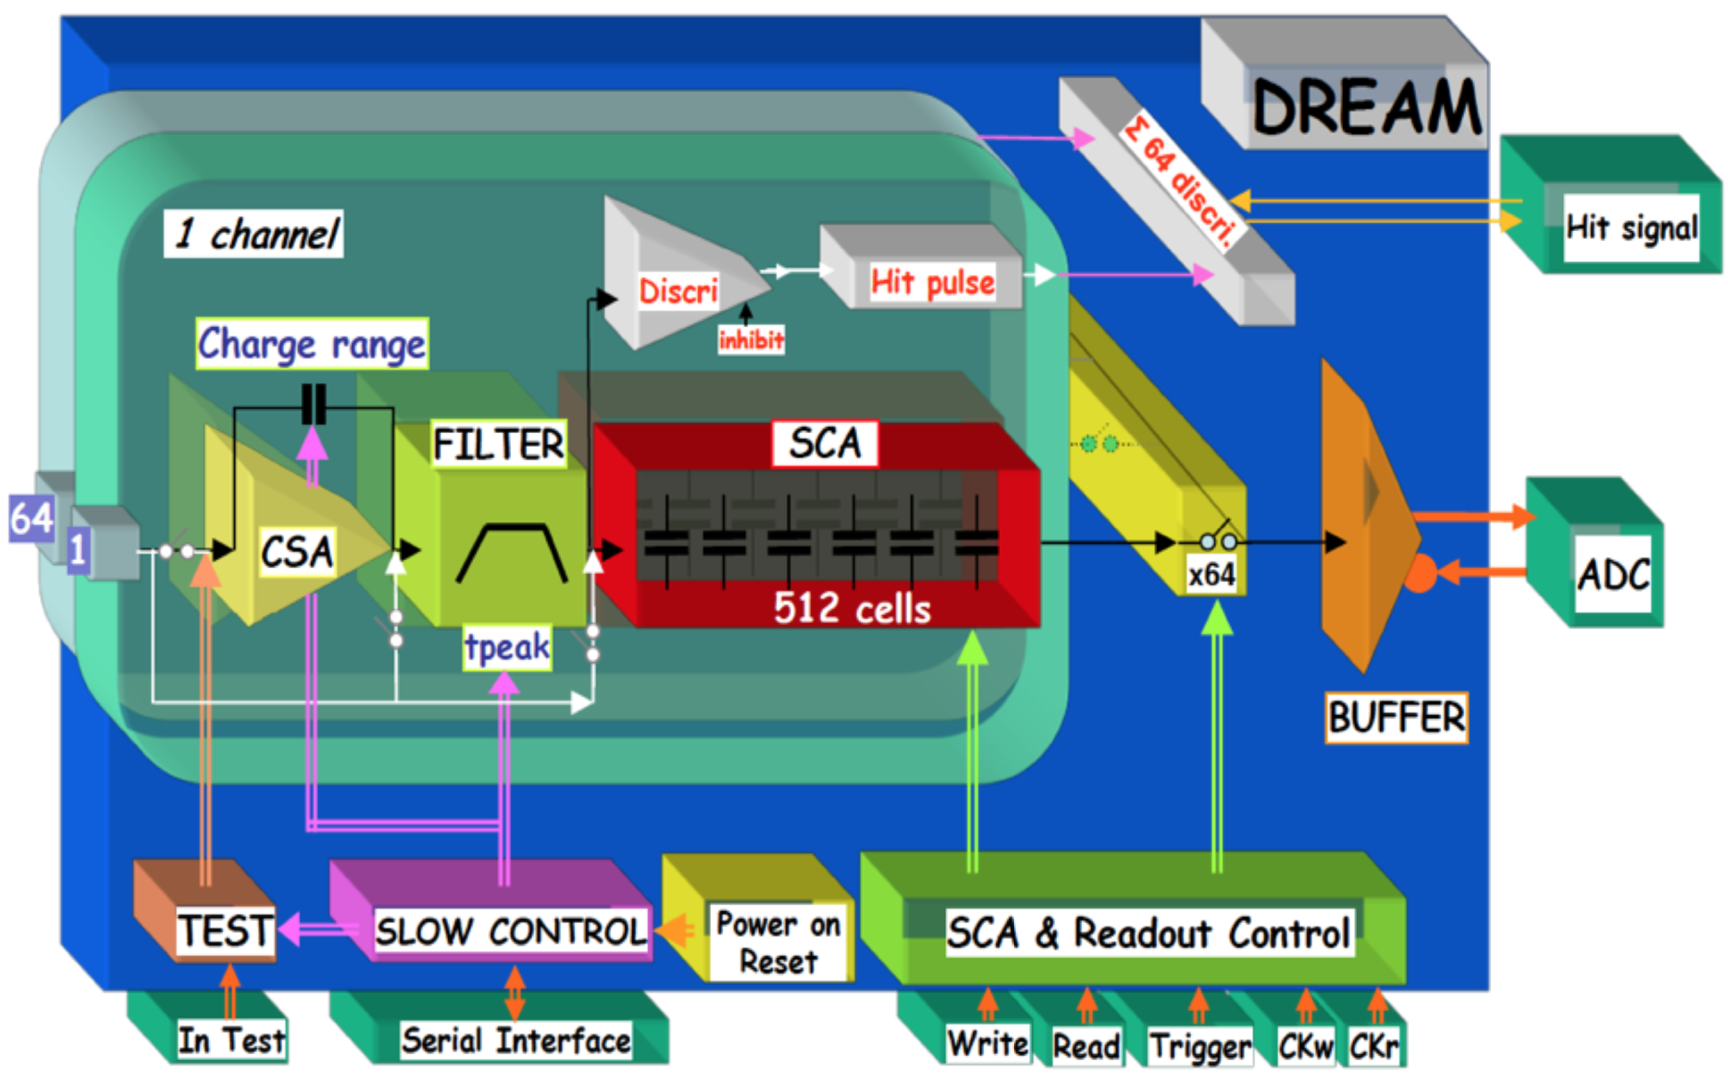
\includegraphics[width=0.6\linewidth]{figures/DREAM_map.png}
	\caption[Map of the DREAM chip.]{Map of the DREAM chip \cite{dream}.}
	\label{fig:dreamn}
\end{figure}

The BONuS12 front-end unit (FEU) utilized the same electronics as the Microgemas Vertex Tracker, which was a detector removed to make room for the BONuS12 RTPC. The FEU contains 8 DREAMs (512 channels), 12-bit 8-channel Analog to Digital Converters (ADCs), Xilinx Virtex-6 FPGA connectivity kits, 2 Mb static RAM, SFP optical transceiver, and a trigger interface. The FEU electronics then drives the signal to the CLAS12 data acquisition system \cite{clas12:data}, which stores the data for analysis. Fig. \ref{fig:rtpc_daq} shows the RTPC DAQ map from signal to back end unit data storage.

\begin{figure}[h!]
	\centering
	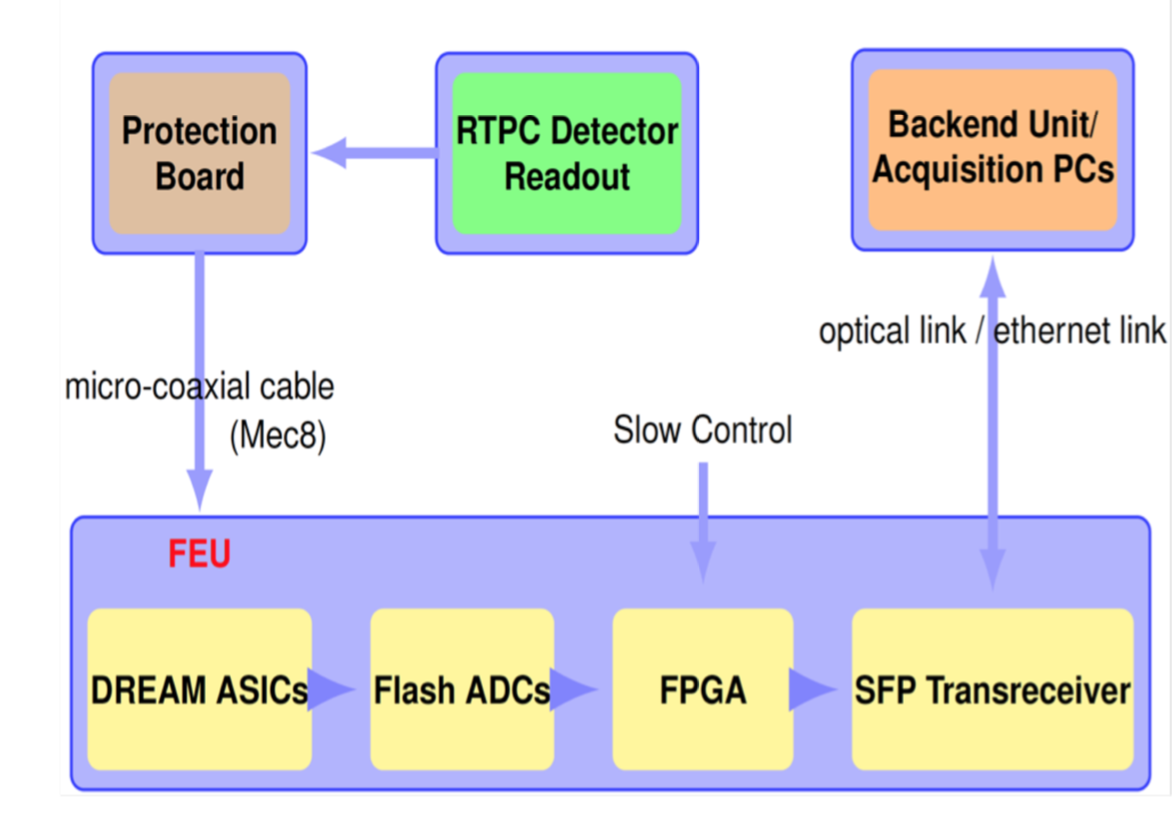
\includegraphics[width=0.6\linewidth]{figures/rtpc_daq.png}
	\caption{The BONuS12 data acquisition map. Signals from the readout pad board go through the translation boards to the front-end unit electronics. The raw events get read into the slow controls and gets uploaded to the back end unit computer systems.}
	\label{fig:rtpc_daq}
\end{figure}

\subsection{RTPC Construction and Integration}
The construction of the BONuS12 RTPC began at Hampton University in Hampton, Virginia around 2017. Because of the cylindrical shape of the detector, mandrels were used widely in the shaping of the detector components. The ground foil, cathode foil, the three layers of GEM foils, and pad board were all assembled using mandrels. Fig. \ref{fig:rtpc_assembly} is a drawing of the assembly station for the RTPC, which includes an actuator that removes wrapped foils from the mandrel and places into the detector on the assembly station.

\begin{figure}[h!]
	\centering
	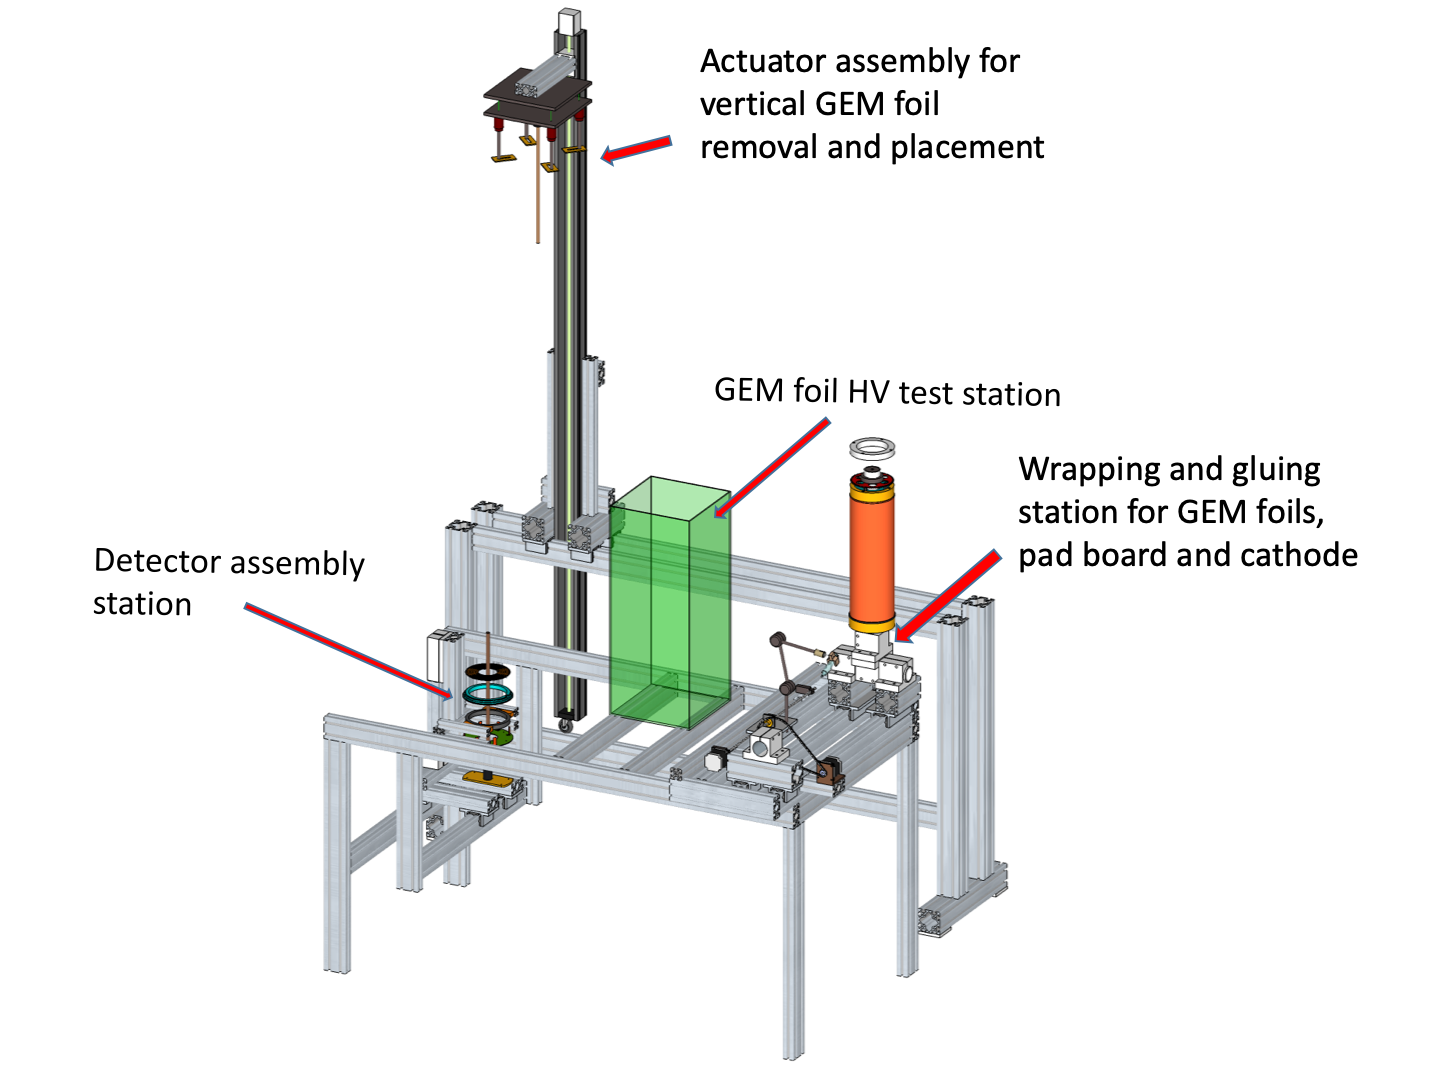
\includegraphics[width=0.8\linewidth]{figures/rtpc_assembly.png}
	\caption{Assembly station for the RTPC.}
	\label{fig:rtpc_assembly}
\end{figure}

The first assembled detector (RTPC1) was delivered to JLab in November 2019. The RTPC underwent testing with cosmic rays in the Experimental Equipment Lab (EEL) at JLab with the full array of components that were eventually installed in the Experimental Hall ($i.e.$ RTPC, gas panel including the Drift-gas Monitoring System, DAQ, etc). 

Once that testing was complete, in late January 2020 the BONuS12 RTPC was installed in Hall B. Run Group F, of which the BONuS12 experiment is a part, required installation of three layers of the Forward Micromegas Tracker (FMT).\footnote{The FMT was originally a part of the Micromegas Vertex Tracker (MVT), which consisted of the FMT and Barrel Micromegas Tracker(BMT). Together the FMT and BMT were designed to improve upon the baseline CLAS12 tracking capabilities.\cite{clas12:MVT} Originally, the FMT contained 6 disks placed 30 cm downstream of the target. For the RGF setup, 3 of those FMT disks were used and the BMT was completely removed to make room for the RTPC.} The support shell and FEUs of the Micromegas were utilized since it allows all electronics to sit outside of the strong solenoid magnetic field.\cite{clas12:MVT} The Forward Tagger required switching to the FTOff condition, which included placing a M\o ller shield in front of the FT.\cite{clas12:FT} After all detector installation was complete in Hall B, cosmic tests were done again. This data stream, for the first time, allowed for the RTPC from within the CLAS12 to be utilized in the full Data Acquisition System \cite{clas12:data} while inside the hall.
\begin{figure}[h!]
	\centering
	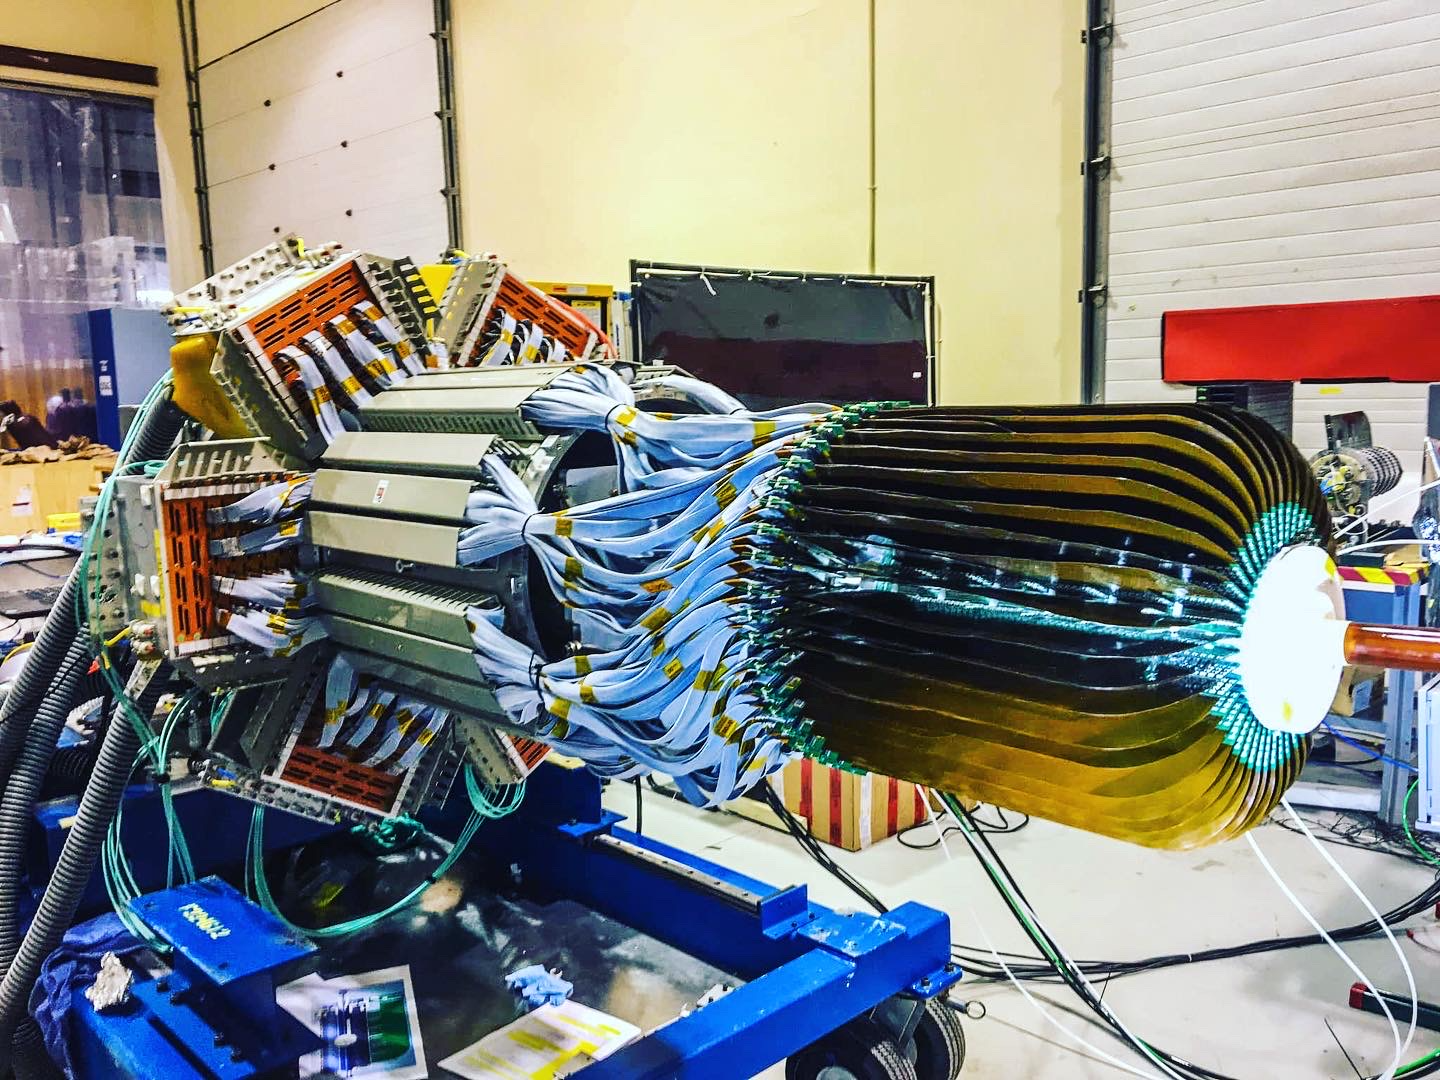
\includegraphics[width=0.95\linewidth]{figures/rtpc_complete.png}
	\caption{The fully assembled BONuS12 RTPC with the FEUs attached, but not yet with the 3-layer FMTs attahced.}
	\label{fig:rtpc_complete}
\end{figure}

\cleardoublepage
\subsection{BONuS12 Drift-gas Monitoring System}
\label{sec:dms}
\begin{wrapfigure}{R}{0.5\linewidth}
	\centering
	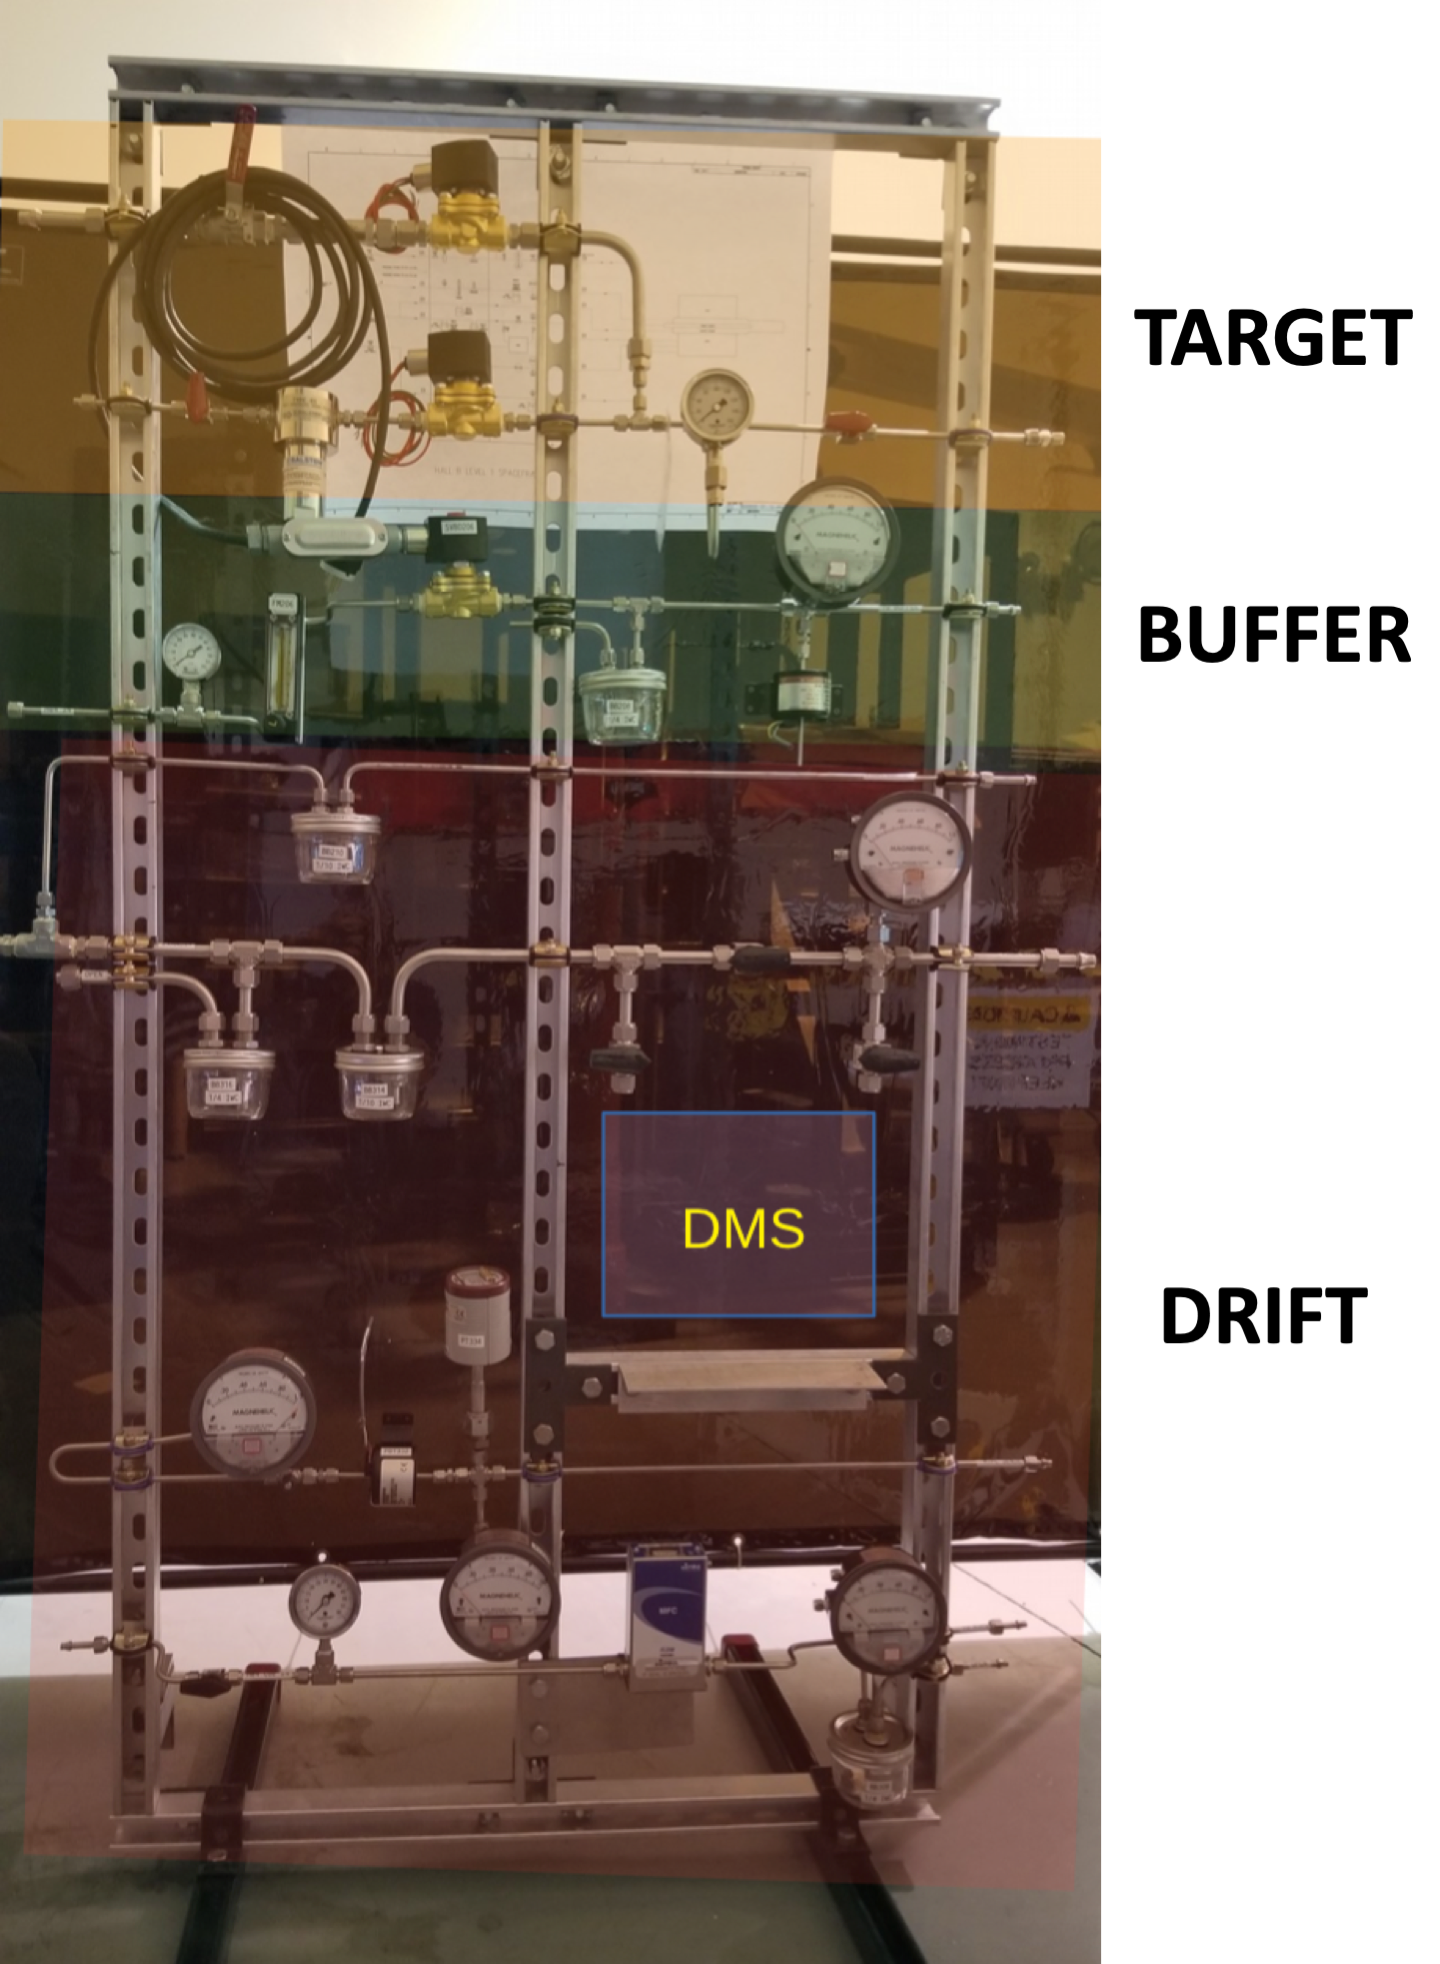
\includegraphics[width=0.9\linewidth]{figures/rtpc_gas_panel.png}
	\caption{\label{fig:rtpc_gas_panel}The RTPC gas panel. The target gas flows through the top part of the panel, the buffer gas flows through the middle region of the panel, and the drift gas flows through the bottom region of the panel.}
\end{wrapfigure}
The gas system for BONuS12 provides gases for the target (deuterium), the buffer regions (helium), and drift region (He:CO2). The gases begin in the gas bottles. The gases travel through the panel seen in Fig. \ref{fig:rtpc_gas_panel}, where the target gas flows through the top, the buffer gas through the middle, and the drift gas through the bottom of the panel. The flow rate is set by Mass Flow Controllers (MFCs) controlled through the CLAS12 slow-control interface Experimental Physics Industrial Control System (EPICS). Once the gas goes through gas-relief bubblers, it enters the RTPC. After flowing through the RTPC, the target and buffer gases goes back through the gas panel and out through exhaust ports. The drift gas exits the RTPC and enters the gas panel into the RTPC Drift-gas Monitoring System (DMS).

The drift velocity of electrons in the RTPC are very sensitive to fluctuations in the gas-mixture and electric field, as well as the temperature and pressure of the gas in the drift region (see \ref{sec:gas_opt}). Therefore, a system was designed that monitors the drift velocity of electrons. A small drift chamber was built that sat downstream of the RTPC and was fed by the drift gas coming from the RTPC.

Since the purpose of the DMS was to measure the drift velocity within the gas mixture, the focus of the DMS design was measuring that velocity through a near-constant electric field. The design concept (seen in Fig. \ref{fig:dms_concept}) is a drift chamber. Two radioactive sources separated by 4 cm emit $\beta$ electrons that are detected by associated scintillator/photomultiplier tubes (PMTs). When these electrons travel through the gas, they create ionization electrons along their path. Within a sensitive region in the center of the DMS, those ionization electrons are guided to an anode wire behind a small slit in a grounded plate by an electric field. 

\begin{figure}[h!]
	\centering
	\includegraphics[width=0.8\linewidth]{figures/dms_concept.png}
	\caption{Design concept of the Drift-gas Monitoring System (DMS) for the BONuS12 experiment.}
	\label{fig:dms_concept}
\end{figure}

The electric field that guides the ionization electrons to the anode is created by a cathode with a high negative potential, an anode with a high positive potential, and field-shaping electrodes that have potentials stepped down by equal amounts from a voltage-divider circuit. This ensures the field within that sensitive region is uniform, so the drift velocity is constant between the two sources.

The DMS outer structure was made from the synthetic polymer called Delrin. Each piece was made on a CNC machine to fit the specifications required. Appendix \ref{apdx:A} contains all drawings and specifications of the DMS. The electrodes (specifications also found in Appendix \ref{apdx:A}) were made from steel. Once the parts were machined, they were assembled in such a way as to leave the stringing of the anode wire last. Each side of the DMS was held together by plastic screws. Fig. \ref{fig:dms_const1} shows the partial construction of the DMS without the last face attached, so the electrodes and cathode exposed. The Photonis XP 2979 PMTs were held in place using a custom built plastic support system (see in Fig \ref{fig:dms_const2} as the black structure with black PMT tubes on the right side). The two 2 \textmu Ci sources were held in place using a Delrin plate. The 30 \textmu m anode wire was strung and crimped. 

\begin{figure}[H]
	\centering
	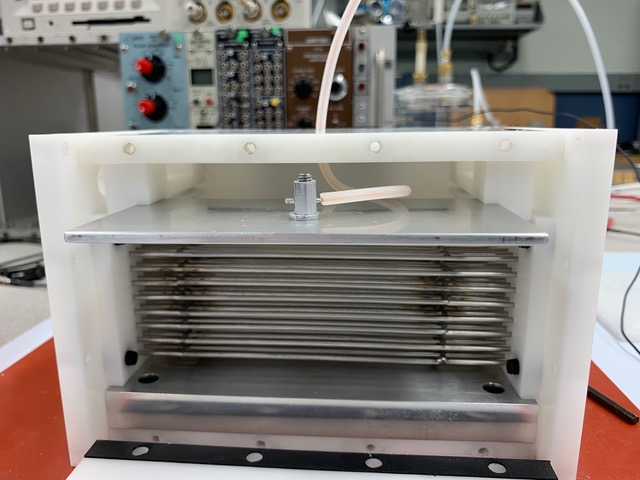
\includegraphics[width=0.75\linewidth]{figures/dms/const1.png}
	\caption{Partial assembly of the DMS showing the wired cathode at the top and the anode ground plate at the bottom with the field shaping electrodes in between.}
	\label{fig:dms_const1}
\end{figure}
\begin{figure}[H]
	\centering
	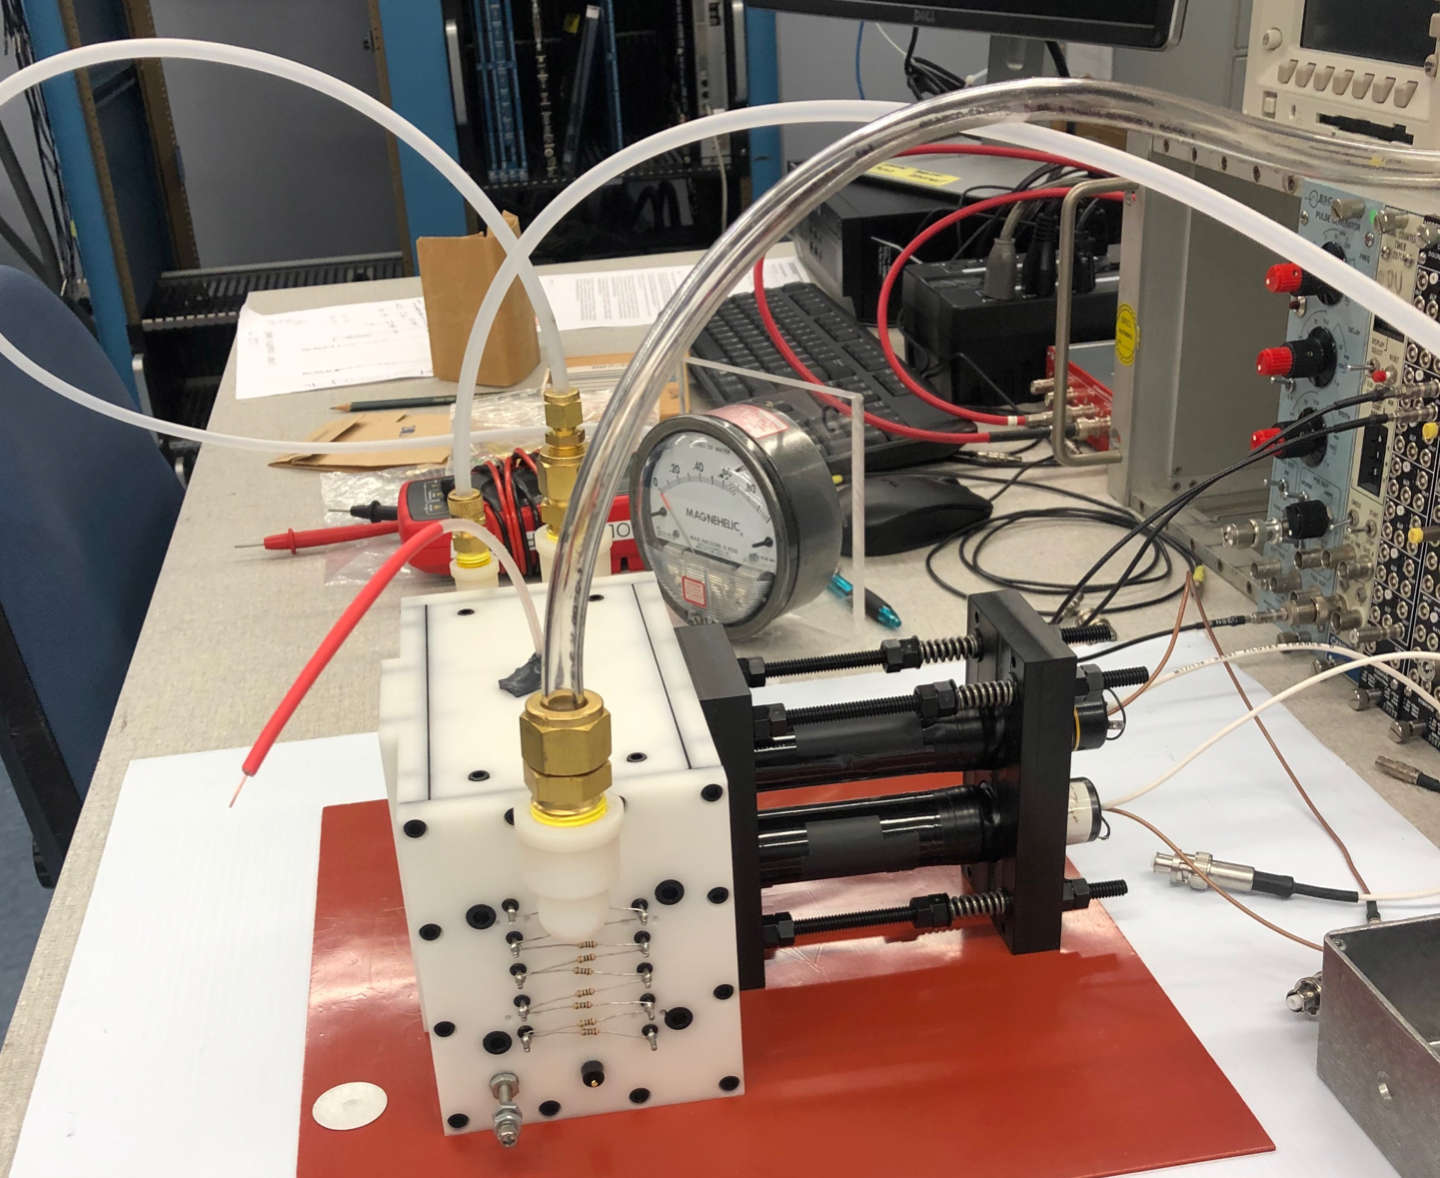
\includegraphics[width=0.75\linewidth]{figures/dms/const2.png}
	\caption{Assembled DMS with electrode wiring.}
	\label{fig:dms_const2}
\end{figure}
\begin{figure}[h!]
	\centering
	\includegraphics[width=0.6\linewidth]{figures/dms/dms_complete.png}
	\caption{Fully assembled DMS with electronics panel shown in the back.}
	\label{fig:dms_const3}
\end{figure}

In order to block any background electromagnetic noise, the entire system was placed in a metal grounded box (see Fig. \ref{fig:dms_const3}). The high-voltage (HV) supply circuits seen in Figs. \ref{fig:dms_cath_circuit} and \ref{fig:dms_anode_circuit} were designed to filter out any fluctuations in the HC supplies. Both circuits were soldered on separate circuit boards and placed on a grounded metal plate along with the preamp/postamp circuit. That grounded plate was screwed to the back of the grounded box and can be seen in the back of the box in Fig. \ref{fig:dms_const3} behind the DMS.

\begin{figure}[h!]
	\centering
	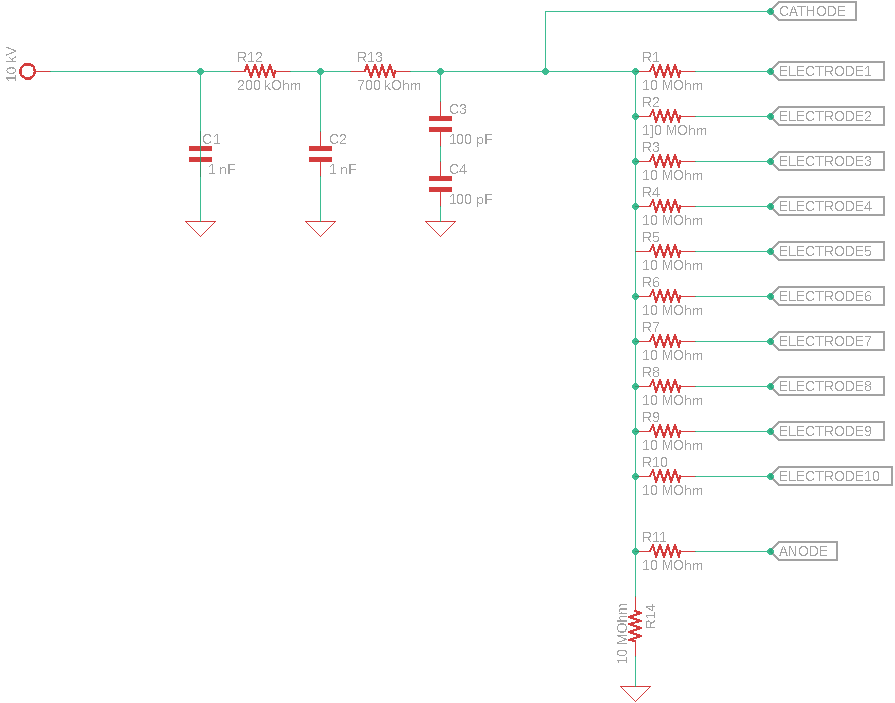
\includegraphics[width=0.99\linewidth]{figures/dms/electrode_supply.png}
	\caption{Cathode and electrode HV supply circuit.}
	\label{fig:dms_cath_circuit}
\end{figure}
\begin{figure}[h!]
	\centering
	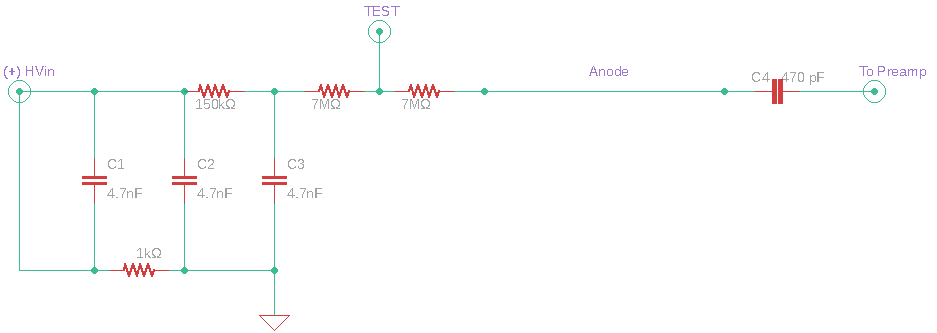
\includegraphics[width=0.99\linewidth]{figures/dms/anode_supply.png}
	\caption{Anode HV supply circuit.}
	\label{fig:dms_anode_circuit}
\end{figure}
\begin{figure}[h!]
	\centering
	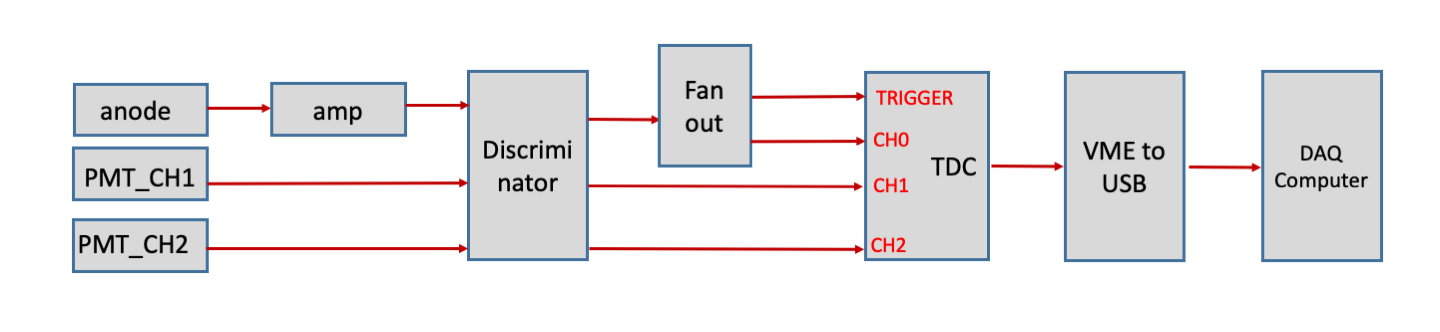
\includegraphics[width=0.95\linewidth]{figures/dms/DAQ_flowchart.png}
	\caption{The DMS DAQ flow from signal to computer.}
	\label{fig:dms_daqflow}
\end{figure}

When a signal is detected at the anode (the trigger), a Time-to-Digital Converter (TDC) (see Fig. \ref{fig:dms_daqflow} for the DMS DAQ map) looks for an associated signal from a source $\beta$ electron detected by either PMT (the PMT closest to the anode is channel 1 and the PMT farthest is channel 2) and measures the time difference between the two signals. When a coincidence occurs, the time difference between trigger and the associated PMT signal is then added to a histogram. As enough statistics populate the histogram, two peaks formed representing events from the two sources and a difference in the two times can be calculated. Given the known distance between the sources and the time difference between the two peaks, the drift velocity is calculated:
\begin{equation}
v_{\mathrm{drift}} = \frac{\Delta d}{\Delta t} = \frac{4 \; \mathrm{cm}}{t_{\mathrm{CH2}} - t_{\mathrm{CH1}}},
\end{equation}
where $v_{\mathrm{drift}}$ is the drift velocity, $\Delta d$ is the distance between sources (equal to 4 cm), $t_{\mathrm{CH1}}$ and $t_{\mathrm{CH2}}$ are the mean values of the Gaussian fits to the peaks from channel 1 and channel 2 respectively. The error on the drift velocity is calculated by
\begin{equation}
\sigma_v = \frac{\sqrt{\sigma_{\mathrm{tCH1}}^2 + \sigma_{\mathrm{tCH1}}^2}}{t_{\mathrm{CH2}} - t_{\mathrm{CH1}}},
\end{equation}
where $\sigma_{\mathrm{tCH1}}$ and $\sigma_{\mathrm{tCH2}}$ are the sigmas on the Gaussian fits for channel 1 and channel 2 respectively. Then the drift velocity is plotted versus elapsed time, giving a means to monitor that velocity.